\documentclass{beamer}
%
% Choose how your presentation looks.
%
% For more themes, color themes and font themes, see:
% http://deic.uab.es/~iblanes/beamer_gallery/index_by_theme.html
%
\mode<presentation>
{
  \usetheme{default}      % or try Darmstadt, Madrid, Warsaw, ...
  \usecolortheme{default} % or try albatross, beaver, crane, ...
  \usefonttheme{default}  % or try serif, structurebold, ...
  \setbeamertemplate{navigation symbols}{}
  \setbeamertemplate{caption}[numbered]
  \setbeamertemplate{footline}[frame number]
} 

\usepackage[english]{babel}
\usepackage[utf8]{inputenc}
\usepackage[T1]{fontenc}
\usepackage{tikz}
\usetikzlibrary{shapes.geometric,arrows}
\usepackage{pgfplots} % For Tikz
% Package for adding comments add disable in [] to remove all comments
%\usepackage[]{todonotes}
\usepackage{amssymb,amsmath}
\usefonttheme{professionalfonts}

\title[Performance Analysis of Source-Seeking Algorithms with Integral Quadratic Constraints]{Performance Analysis of Source-Seeking Algorithms with Integral Quadratic Constraints}
\author{Adwait Datar}
\institute{PhD Workshop, 2021\\Technical University of Hamburg}
\date{$28^{th}$ Feb, 2022}

\begin{document}

\begin{frame}	
  \titlepage
\end{frame}
%%%%%%%%%%%%%%%%%%%%%%%%%%%%%%%%%%%%%%%%%%%%%%%%%%%%%%%%%%%%%%%%%%%%%
\begin{frame}{Source-seeking Problem}
	\begin{figure}[!htb]
		\centering
		\begin{minipage}{.5\textwidth}
			\centering
			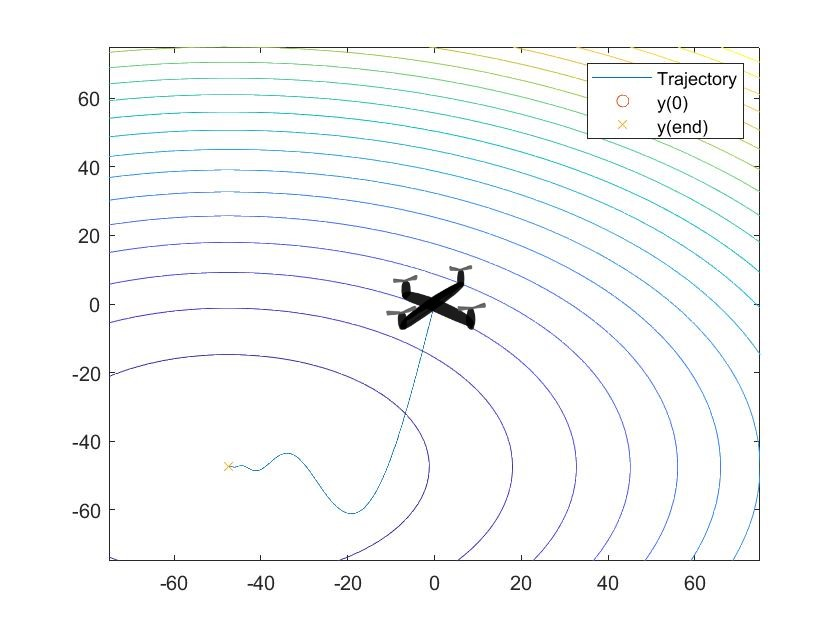
\includegraphics[width=0.9\linewidth,height=0.45\textheight]{figures/single_quad_field.jpg}
			%\caption{Single quadrotor}
			\label{fig:single_quad}
			PhD workshop Sept 2021
		\end{minipage}%
		\begin{minipage}{0.5\textwidth}
			\centering
			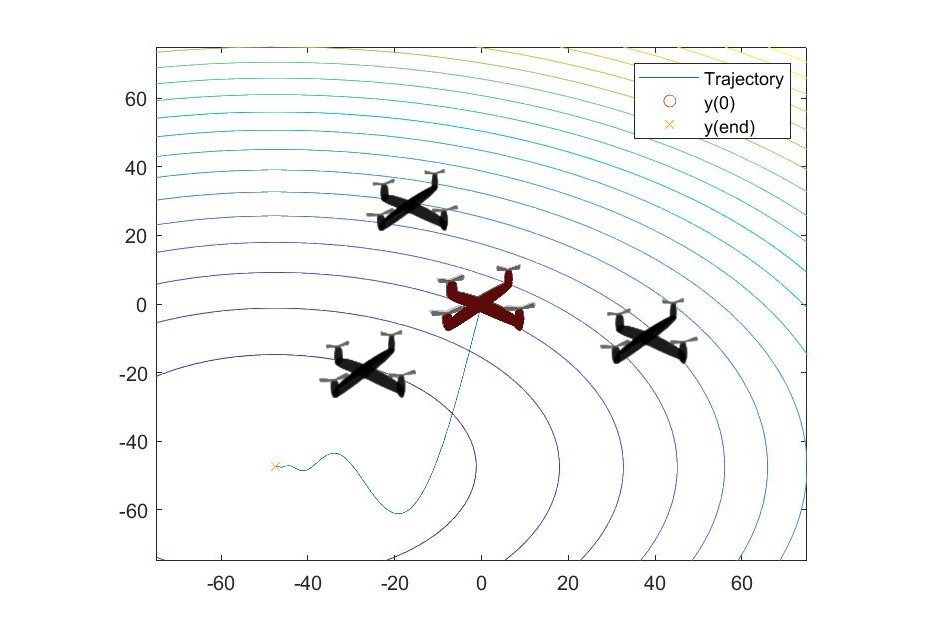
\includegraphics[width=0.9\linewidth,height=0.45\textheight]{figures/multiple_quad_field.jpg}
			%\caption{Multiple quadrotors}
			\label{fig:multiple_quads}
			PhD workshop Feb 2022
		\end{minipage}
		\end{figure}
	\begin{block}{Assumptions (Informal)}
		\begin{itemize}		
			\item Field is differentiable and convex
			\item Local gradients available at \textcolor{red}{some} leader agents 
			\item Connectivity assumptions on interconnection graphs
		\end{itemize}		
	\end{block}
\end{frame}

% Uncomment these lines for an automatically generated outline.
\begin{frame}{Outline}
	\tableofcontents
\end{frame}
%%%%%%%%%%%%%%%%%%%%%%%%%%%%%%%%%%%%%%%%%%%%%%%%%%%%%%%%%%%%%%%%%%%%%
\section{Review: Single agent case}
%%%%%%%%%%%%%%%%%%%%%%%%%%%%%%%%%%%%%%%%%%%%%%%%%%%%%%%%%%%%%%%%%%%%%
%\begin{frame}{Motivations and relevant works}
%	\begin{block}{Earlier work on analysis of source-seeking algorithms}
%	\begin{itemize}
%		\item Stability analysis but no performance guarantees [Attallah, 2020], [Datar, Paulsen and Werner, 2020]
%		\item Lyapunov (storage) functions are constructed based on physically motivated energy like functions: Diagonal Lyapunov (storage) functions [Datar, Paulsen and Werner, 2020]
%		\item Use small-gain arguments for general non-linear (LPV) agents [Attallah, Datar and Werner, 2020]
%	\end{itemize}
%	\end{block}	
%	\begin{block}{Key contributions of this work}
%	\begin{itemize}
%		\item Performance analysis with guaranteed rates of convergence
%		\item Quantifiable robustness w.r.t underlying field
%		\item Less conservative results with dynamic non-causal multipliers
%	\end{itemize}
%\end{block}
%\end{frame}
%%%%%%%%%%%%%%%%%%%%%%%%%%%%%%%%%%%%%%%%%%%%%%%%%%%%%%%%%%%%%%%%%%%%%
\begin{frame}{Control Architecture: Single Agent}
\begin{figure}[ht]
	\tikzstyle{block} = [draw, rectangle, 
    minimum height=3em, minimum width=6em]
\tikzstyle{sum} = [draw,  circle, node distance=1cm]
\tikzstyle{input} = [coordinate]
\tikzstyle{output} = [coordinate]
\tikzstyle{pinstyle} = [pin edge={to-,thin,black}]

% The block diagram code is probably more verbose than necessary
%\begin{tikzpicture}[auto, node distance=2cm,>=latex']
%    % We start by placing the blocks
%    \node [input, name=input] {};
%    \node [sum, right of=input] (sum) {};
%    \node [block, right of=sum] (controller) {Controller};
%    \node [block, right of=controller, pin={[pinstyle]above:Disturbances},
%            node distance=3cm] (system) {System};
%    % We draw an edge between the controller and system block to 
%    % calculate the coordinate u. We need it to place the measurement block. 
%    \draw [->] (controller) -- node[name=u] {$u$} (system);
%    \node [output, right of=system] (output) {};
%    \node [block, below of=u] (measurements) {Measurements};
%
%    % Once the nodes are placed, connecting them is easy. 
%    \draw [draw,->] (input) -- node {$r$} (sum);
%    \draw [->] (sum) -- node {$e$} (controller);
%    \draw [->] (system) -- node [name=y] {$y$}(output);
%    \draw [->] (y) |- (measurements);
%    \draw [->] (measurements) -| node[pos=0.99] {$-$} 
%        node [near end] {$y_m$} (sum);
%\end{tikzpicture}

\begin{tikzpicture}[auto, node distance=2cm,>=latex']
% We start by placing the blocks
\node [input, name=input] {};
\node [block, right of=input,node distance=3cm](Flockcontrol) {$\begin{array}{cc}
   \Dot{q} =& p \\
   \Dot{p} =&-k_d p-k_p u
\end{array}$};
\node [block, right of=Flockcontrol,node distance=4cm,minimum height=2.5em,minimum width=3em](velocityloop) {$\left[\begin{array}{c|c}
A     &  B\\
\hline
C     &  \mathbf{0}
\end{array}\right]$};
\node [output, right of=velocityloop,node distance=1.4cm](output) {};
\node [block, below of=Flockcontrol,node distance=2cm](delta) {$u=\nabla f(y)$};
\node[text=red, above of = Flockcontrol,xshift=-2cm,yshift=-0.5cm] (veh) {$G$};
\draw[red, dashed] (veh.east)-|([xshift=-3.8mm]output.west)|-([yshift=-3mm]Flockcontrol.south)-|([xshift=2mm]input.west)|-(veh.west);
% Once the nodes are placed, connecting them is easy. 
\draw [draw,->] (input) -- node {$u$} (Flockcontrol);
\draw [draw,->] (Flockcontrol) -- node {$\begin{bmatrix}q\\p\end{bmatrix}$} (velocityloop);
\draw [draw,->] (velocityloop) -- node[name=outmid] {$y$} (output);
\draw [->] (outmid) |- (delta);
\draw [-] (delta) -| (input);
\end{tikzpicture}
	%\caption{Control architecture}
	\label{fig:control_architecture}	
\end{figure}
%	\begin{figure}[t]
%		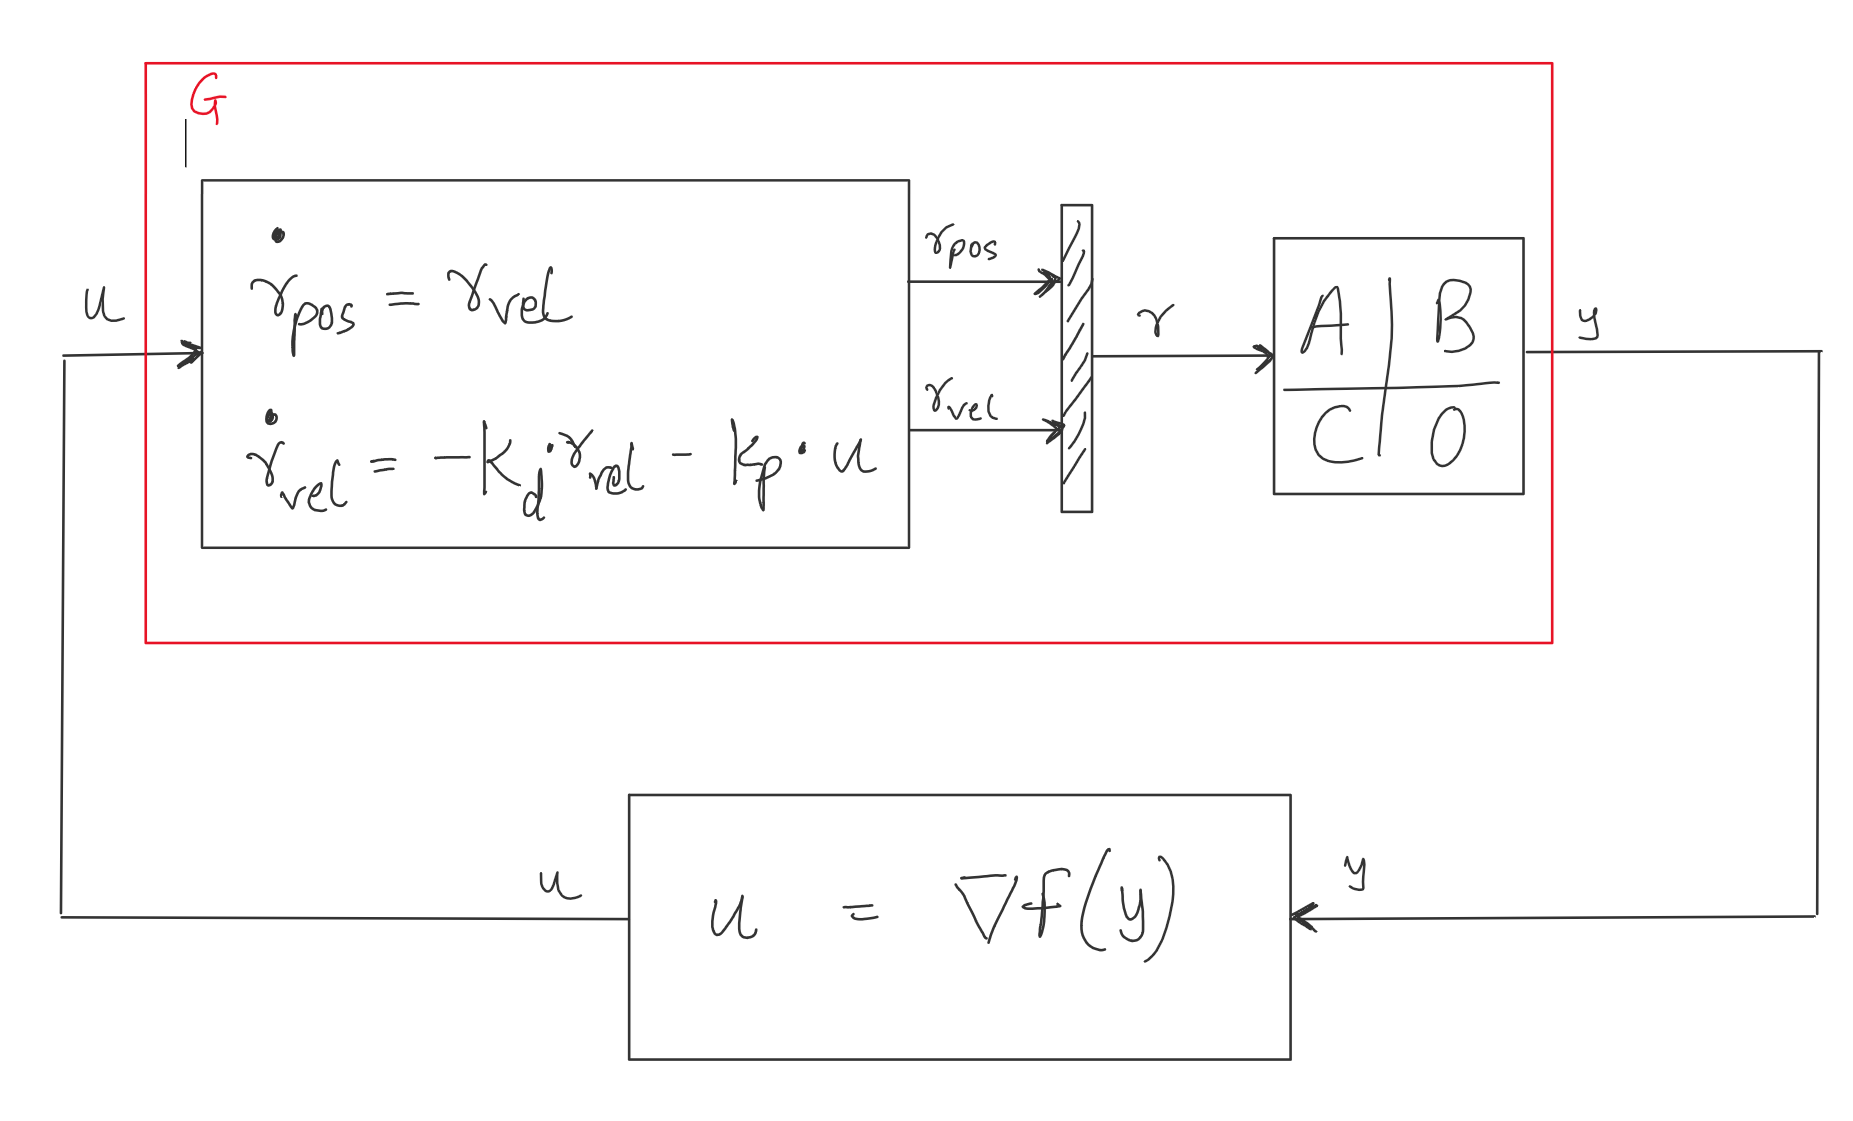
\includegraphics[width=8cm]{figures/Figure_IQC_paper.PNG}
%		%\input{figures/quadrotor_trajectory}
%		%\caption{Block diagram}
%		\centering
%		\label{fig:Figure_IQC_paper}
%	\end{figure}
	\begin{equation*} \label{eq:sys_dyn_G}
		\begin{split}
			\Dot{\eta}(t)&=A_G\eta(t) + B_G u(t), \quad \quad \eta(0)=\eta_0\\
			y(t)&=C_G \eta(t) \\
			u(t)&=\nabla f(y(t)),
		\end{split}
	\end{equation*}
\end{frame}
%%%%%%%%%%%%%%%%%%%%%%%%%%%%%%%%%%%%%%%%%%%%%%%%%%%%%%%%%%%%%%%%%%%%%
\begin{frame}{Loop in the deviation variables: Single agent}
	\begin{block}{Equilibrium}
		\begin{equation} \label{eq:sys_dyn_G_delta}
			\begin{split}
				0&=A_G\eta_* + B_G u_*=A_G\eta_*\\
				y&=C_G \eta_*\\
				u_*&=\nabla f(y_*)=0
			\end{split}
		\end{equation}
	\end{block}
	\begin{block}{Loop in the transformed variables}
		\begin{equation} \label{eq:sys_dyn_G_tilde}
			\begin{split}
				\Dot{\Tilde{\eta}}(t)&=A_G\Tilde{\eta}(t) + B_G \Tilde{u}(t), \quad \quad \Tilde{\eta}(0)=\eta_0-\eta_*\\
				\Tilde{y}(t)&=C_G \Tilde{\eta}(t)
			\end{split}
		\end{equation}
		and 
		\begin{equation} \label{eq:delta}
			\Tilde{u}(t)=\nabla f(\Tilde{y}(t)+y_*)
		\end{equation}
	\end{block}
\end{frame}
%%%%%%%%%%%%%%%%%%%%%%%%%%%%%%%%%%%%%%%%%%%%%%%%%%%%%%%%%%%%%%%%%%%%%
\begin{frame}{Main Results: Single Agent}
		\begin{itemize}
			\item Let $y_*$ minimizes $f\in \mathcal{S}(m,L)$
			\footnote{$m||y_1-y_2||^2 \leq  (\nabla f(y_1)-\nabla f(y_2))^T(y_1-y_2) \leq L ||y_1-y_2||^2$} 
			\pause
			\item $\left[\begin{array}{c|c}
				\mathcal{A}     &  \mathcal{B}\\
				\hline
				\mathcal{C}     &  \mathcal{D}
			\end{array}\right]=\Pi \begin{bmatrix}
			G\\
			I_{d}
		\end{bmatrix}
			\pause 
			=
			\left[
			\begin{array}{c|c}
			A_{\pi} \otimes I_{d} & B_{\pi} \otimes I_{d} \\
			\hline
			C_{\pi} \otimes I_{d} & D_{\pi} \otimes I_{d}
		\end{array}
	\right]\left[
	\begin{array}{c|c}
		A_{G} & B_{G} \\
		\hline
		C_{G} 		& \mathbf{0} \\
		\mathbf{0} 	& I_d
	\end{array}
	\right]$
			\pause 
			\item $\mathbb{P}=\left\{
			\begin{bmatrix}
				\mathbf{0}  & \begin{bmatrix}
					H  & -P_3 \\
					-P_1^T    & \mathbf{0}
				\end{bmatrix} \\
				*    & \mathbf{0}
			\end{bmatrix}: \textnormal{LMI}(H,P_1,P_3)<0
			\right\}$
		\end{itemize}
	\pause 
	\begin{block}{Theorem 1}
		If $\exists \mathcal{X}>0,P \in \mathbb{P}$ such that
		\begin{equation*}%\label{eq:perf_LMI}
			\begin{bmatrix}
				\mathcal{A}^T\mathcal{X}+\mathcal{X}\mathcal{A}+2\alpha \mathcal{X}  & \mathcal{X}\mathcal{B} \\
				\mathcal{B}^T\mathcal{X}    & \mathbf{0}
			\end{bmatrix}
			+
			\begin{bmatrix}
				\mathcal{C}^T \\
				\mathcal{D}^T 
			\end{bmatrix}
			( P\otimes I_d)
			\begin{bmatrix}
				\mathcal{C} & \mathcal{D} 
			\end{bmatrix}
			\leq 
			0,
		\end{equation*}
		then, $||y(t)-y_*(t)||\leq \kappa e^{-\alpha t}$ holds for all $t\geq 0$
	\end{block}
\end{frame}
%%%%%%%%%%%%%%%%%%%%%%%%%%%%%%%%%%%%%%%%%%%%%%%%%%%%%%%%%%%%%%%%%%%%%%
%\begin{frame}{Theory}
%	\begin{block}{Relevant Literature}
%		\begin{itemize}
%			\item Exponential IQCs introduced in [Lessard,Recht and Packard, 2016], [Hu and Seiler, 2016], 
%			\item Non-causal dynamic Zames Falb $\alpha$-IQCs [Freeman, 2018] 
%			\item Parameterization of dynamics Zames Falb IQCs [Veenman and Scherer, 2018] 
%		\end{itemize}
%	\end{block}	
%	\begin{block}{theoretical contribution of this work}
%	\begin{itemize}
%		\item Derivation of a general non-causal dynamic $\alpha$-ZF IQCs
%		non-causal dynamic multipliers with an LMI-able parameterization
%	\end{itemize}
%\end{block}	
%\end{frame}

%%%%%%%%%%%%%%%%%%%%%%%%%%%%%%%%%%%%%%%%%%%%%%%%%%%%%%%%%%%%%%%%%%%%%
%\begin{frame}{Loop in the deviation variables}
%	\begin{figure}[!htb]
%		\centering
%		\begin{minipage}{.5\textwidth}
%			\centering
%			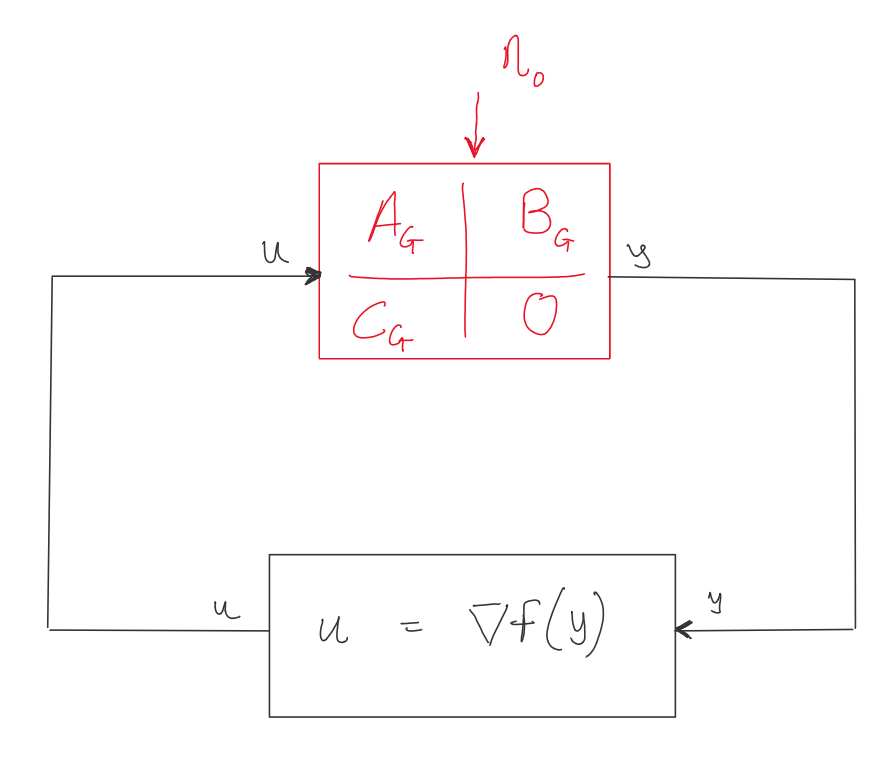
\includegraphics[width=0.8\linewidth,height=0.45\textheight]{figures/loop.PNG}
%			\caption{Original loop}
%			\label{fig:prob1_6_2}
%		\end{minipage}%
%		\begin{minipage}{0.5\textwidth}
%			\centering
%			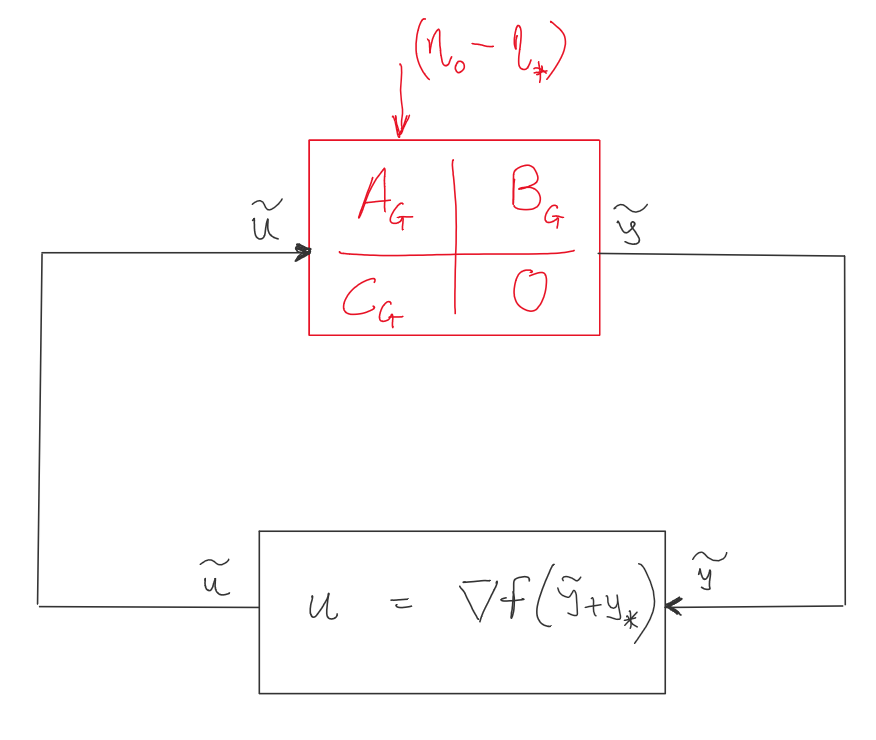
\includegraphics[width=0.8\linewidth,height=0.45\textheight]{figures/loop_dev_vars.PNG}
%			\caption{Loop in deviation variables}
%			\label{fig:prob1_6_1}
%		\end{minipage}
%	\end{figure}
%\begin{block}{Assumption 1}
%	Let $f$ be a differentiable convex field with the minimum at $y_*$ satisfying
%	\begin{equation*}
%		m||y_1-y_2||^2 \leq  (\nabla f(y_1)-\nabla f(y_2))^T(y_1-y_2) \leq L ||y_1-y_2||^2 \quad \forall y_1,y_2.
%	\end{equation*}
%	
%\end{block}
%\end{frame}
%%%%%%%%%%%%%%%%%%%%%%%%%%%%%%%%%%%%%%%%%%%%%%%%%%%%%%%%%%%%%%%%%%%%%
%\begin{frame}{Zames Falb IQCs}	
%	\begin{figure}[t]
%		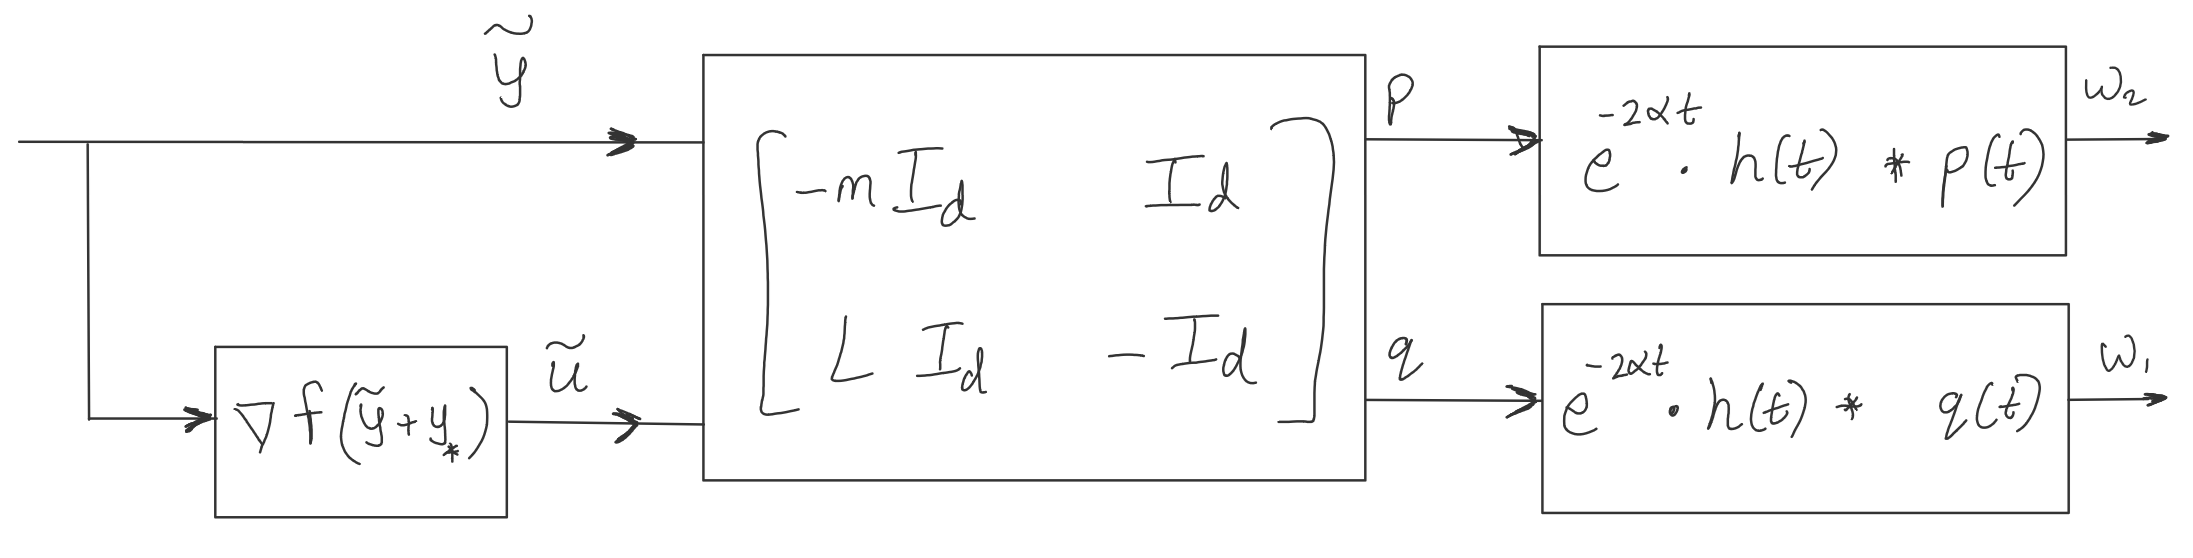
\includegraphics[width=9cm]{figures/signal_definitions_p_q_w.PNG}
%		%\input{figures/quadrotor_trajectory}
%		%\caption{Block diagram}
%		\centering
%		%\label{fig:Figure_IQC_paper}
%	\end{figure}
%\textbf{Theorem:} Let $h \in \mathcal{L}_1(-\infty,\infty)$ satisfy
%		\begin{equation} \label{eq:zf_impulse_resp_cond}
%			\begin{aligned}
%				h(s) &\geq 0, \quad \forall s \in \mathbb{R} \textnormal{ and } \int_{-\infty}^{\infty}h(s)ds &\leq H.
%			\end{aligned}
%		\end{equation}	
%	Then, under the assumptions on $f$, $\forall T \geq 0$ and $\forall \tilde{y} \in \mathcal{L}_{2e}$,	
%		\begin{equation}
%			\int_0^T e^{2\alpha t}( H p(t)^T q(t) - p(t)^T w_1(t) - q(t)^T w_2(t)) dt \geq 0.
%		\end{equation}
%
%\end{frame}
%%%%%%%%%%%%%%%%%%%%%%%%%%%%%%%%%%%%%%%%%%%%%%%%%%%%%%%%%%%%%%%%%%%%%%
%\begin{frame}{Parameterize $h(t)$}	
%	
%\begin{itemize}
%\item Fix $A_{\nu}=
%\begin{bmatrix} 
%	\rho   & 0      &\dots     & 0 \\
%	1      & \rho   & \ddots        &0  \\
%	0      & \ddots      & \ddots     &0  \\
%	\vdots & 0      & 1        &\rho  
%\end{bmatrix},
%B_{\nu}=
%\begin{bmatrix} 
%	1 \\
%	0\\
%	\vdots\\
%	0 
%\end{bmatrix}.$
%\item Parameterize $h(t)$ as  
%\begin{equation}\label{eq:h_defn}
%	\begin{split}
%		h(t)&=
%		\begin{cases}
%			P_1 e^{-A_{\nu}t}B_{\nu}, & \text{if}\ t<0 \\
%			P_3 e^{A_{\nu}t}B_{\nu}, & \text{if}\ t\geq 0
%		\end{cases}
%	\end{split}
%\end{equation}
%\item If $\textnormal{LMI}(H,P_1,P_3)<0$, conditions on $h(t)$ hold [Scherer, 2013].
%\item For searching over only causal(anti-causal) multipleirs, set $P_1=0$ ($P_3=0$)
%\item For searching over static multipliers(Circle criterion), set $P_1=0$ and $P_3=0$
%\end{itemize}
%	
%%	\begin{equation}
%%		A_{\nu}=
%%		\begin{bmatrix} 
%%			\rho   & 0      &\dots     & 0 \\
%%			1      & \rho   & \ddots        &0  \\
%%			0      & \ddots      & \ddots     &0  \\
%%			\vdots & 0      & 1        &\rho  
%%		\end{bmatrix},
%%		B_{\nu}=
%%		\begin{bmatrix} 
%%			1 \\
%%			0\\
%%			\vdots\\
%%			0 
%%		\end{bmatrix}.
%%	\end{equation}
%	
%	
%	
%\end{frame}
%%%%%%%%%%%%%%%%%%%%%%%%%%%%%%%%%%%%%%%%%%%%%%%%%%%%%%%%%%%%%%%%%%%%%
%\begin{frame}{Parameterize $h(t)$}
%\begin{figure}[t]
%	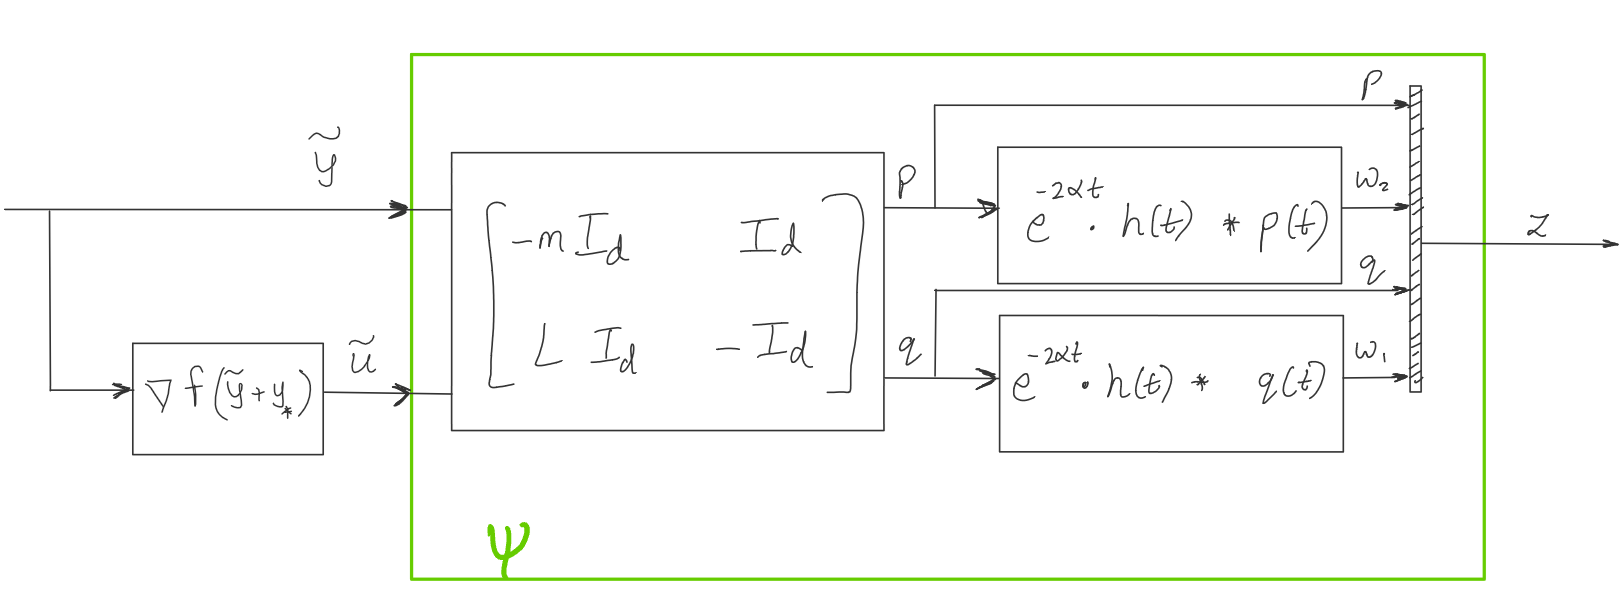
\includegraphics[width=9cm]{figures/signal_definitions.PNG}
%	%\input{figures/quadrotor_trajectory}
%	%\caption{Block diagram}
%	\centering
%	%\label{fig:Figure_IQC_paper}
%\end{figure}
%\begin{equation*}
%	( H p^T q - p^T w_1 - q^T w_2)=		
%	\tilde{z}^T
%	\begin{bmatrix}
%		\mathbf{0}  & \begin{bmatrix}
%			H  & -P_3 \\
%			-P_1^T    & \mathbf{0}
%		\end{bmatrix} \\
%		*    & \mathbf{0}
%	\end{bmatrix}\tilde{z}
%\end{equation*}	
%Define $\mathbb{P}$ such that every $P \in \mathbb{P}$ generates a valid $h(t)$.	
%\begin{equation*}
%	\mathbb{P}=\left\{
%	\begin{bmatrix}
%		\mathbf{0}  & \begin{bmatrix}
%			H  & -P_3 \\
%			-P_1^T    & \mathbf{0}
%		\end{bmatrix} \\
%		*    & \mathbf{0}
%	\end{bmatrix}: \textnormal{LMI}(H,P_1,P_3)<0
%	\right\}
%\end{equation*}
%
%
%%Let the state space realization of $\Psi$ be 
%%\begin{equation}\label{eq:ss_Psi}
%%	\left[
%%	\begin{array}{c|c}
%%		A_{\Psi} & B_{\Psi} \\
%%		\hline
%%		C_{\Psi} & D_{\Psi}
%%	\end{array}
%%	\right]
%%	=
%%	\left[
%%	\begin{array}{cc|cc}
%%		A_{\nu}^{\alpha} \otimes I_d        &\mathbf{0}                         &-B_{\nu}\otimes mI_d       &B_{\nu}\otimes I_d \\
%%		\mathbf{0}                          &A_{\nu}^{\alpha} \otimes I_d       &B_{\nu}\otimes LI_d        &-B_{\nu}\otimes I_d \\
%%		\hline
%%		\mathbf{0}                          &\mathbf{0}                         &-mI_d                      &I_d \\
%%		I_{\nu}\otimes I_d                  &\mathbf{0}                         &\mathbf{0}                 &\mathbf{0}\\
%%		\mathbf{0}                          &\mathbf{0}                         &LI_d                       &-I_d\\
%%		\mathbf{0}                          &I_{\nu}\otimes I_d                 &\mathbf{0}                 &\mathbf{0}
%%	\end{array}
%%	\right].
%%\end{equation}
%\end{frame}

%%%%%%%%%%%%%%%%%%%%%%%%%%%%%%%%%%%%%%%%%%%%%%%%%%%%%%%%%%%%%%%%%%%%%
%\begin{frame}{Theory}
%	\begin{figure}[t]
%	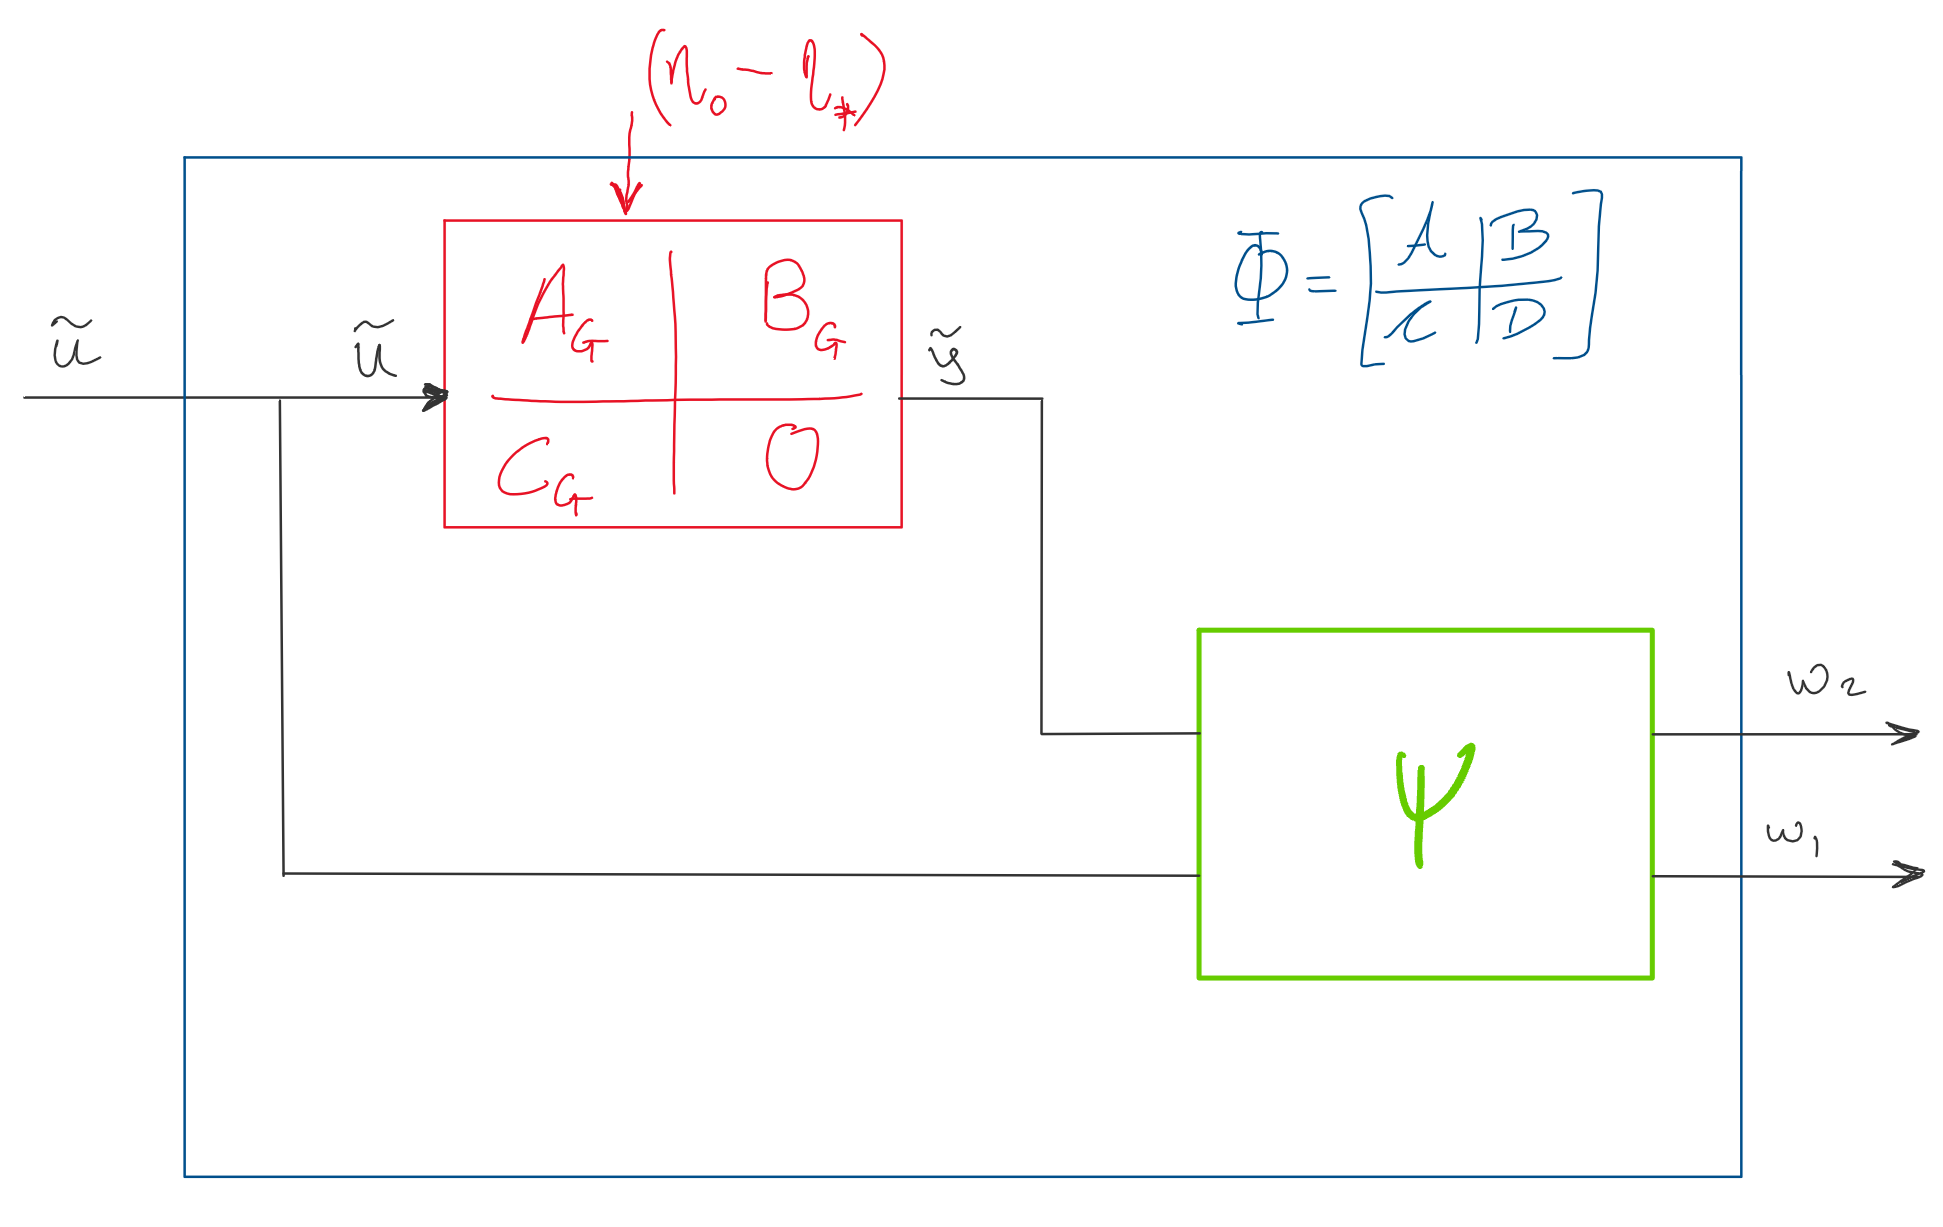
\includegraphics[width=5cm]{figures/Psi_GI.PNG}
%	%\input{figures/quadrotor_trajectory}
%	% \caption{Block diagram}
%	\centering
%	%\label{fig:Figure_IQC_paper}
%	\end{figure}
%\begin{theorem}\label{theom:theorem_perf_analysis}
%	If $\exists \mathcal{X}>0,P \in \mathbb{P}$ such that
%	\begin{equation}\label{eq:perf_LMI}
%		\begin{bmatrix}
%			\mathcal{A}^T\mathcal{X}+\mathcal{X}\mathcal{A}+2\alpha \mathcal{X}  & \mathcal{X}\mathcal{B} \\
%			\mathcal{B}^T\mathcal{X}    & \mathbf{0}
%		\end{bmatrix}
%		+
%		\begin{bmatrix}
%			\mathcal{C}^T \\
%			\mathcal{D}^T 
%		\end{bmatrix}
%		( P\otimes I_d)
%		\begin{bmatrix}
%			\mathcal{C} & \mathcal{D} 
%		\end{bmatrix}
%		\leq 
%		0,
%	\end{equation}
%	then, $y$ converges exponentially to $y_*$ with rate $\alpha$, i.e., $\exists \kappa \geq 0$ such that  
%	$||\Tilde{y}(t)||\leq \kappa e^{-\alpha t}$ holds for all $t\geq 0$.
%\end{theorem}
%\end{frame}
%%%%%%%%%%%%%%%%%%%%%%%%%%%%%%%%%%%%%%%%%%%%%%%%%%%%%%%%%%%%%%%%%%%%%
\begin{frame}{Numerical results for a single quadrotor}
\begin{figure}[ht]
	\tikzstyle{block} = [draw, rectangle, 
    minimum height=3em, minimum width=6em]
\tikzstyle{sum} = [draw,  circle, node distance=1cm]
\tikzstyle{input} = [coordinate]
\tikzstyle{output} = [coordinate]
\tikzstyle{pinstyle} = [pin edge={to-,thin,black}]

% The block diagram code is probably more verbose than necessary
%\begin{tikzpicture}[auto, node distance=2cm,>=latex']
%    % We start by placing the blocks
%    \node [input, name=input] {};
%    \node [sum, right of=input] (sum) {};
%    \node [block, right of=sum] (controller) {Controller};
%    \node [block, right of=controller, pin={[pinstyle]above:Disturbances},
%            node distance=3cm] (system) {System};
%    % We draw an edge between the controller and system block to 
%    % calculate the coordinate u. We need it to place the measurement block. 
%    \draw [->] (controller) -- node[name=u] {$u$} (system);
%    \node [output, right of=system] (output) {};
%    \node [block, below of=u] (measurements) {Measurements};
%
%    % Once the nodes are placed, connecting them is easy. 
%    \draw [draw,->] (input) -- node {$r$} (sum);
%    \draw [->] (sum) -- node {$e$} (controller);
%    \draw [->] (system) -- node [name=y] {$y$}(output);
%    \draw [->] (y) |- (measurements);
%    \draw [->] (measurements) -| node[pos=0.99] {$-$} 
%        node [near end] {$y_m$} (sum);
%\end{tikzpicture}

\begin{tikzpicture}[auto, node distance=2cm,>=latex']
% We start by placing the blocks
\node [input, name=input] {};
\node [block, right of=input,node distance=3cm](Flockcontrol) {$\begin{array}{cc}
   \Dot{q} =& p \\
   \Dot{p} =&-k_d p-k_p u
\end{array}$};
\node [block, right of=Flockcontrol,node distance=4cm,minimum height=2.5em,minimum width=3em](velocityloop) {$\left[\begin{array}{c|c}
A     &  B\\
\hline
C     &  \mathbf{0}
\end{array}\right]$};
\node [output, right of=velocityloop,node distance=1.4cm](output) {};
\node [block, below of=Flockcontrol,node distance=2cm](delta) {$u=\nabla f(y)$};
\node[text=red, above of = Flockcontrol,xshift=-2cm,yshift=-0.5cm] (veh) {$G$};
\draw[red, dashed] (veh.east)-|([xshift=-3.8mm]output.west)|-([yshift=-3mm]Flockcontrol.south)-|([xshift=2mm]input.west)|-(veh.west);
% Once the nodes are placed, connecting them is easy. 
\draw [draw,->] (input) -- node {$u$} (Flockcontrol);
\draw [draw,->] (Flockcontrol) -- node {$\begin{bmatrix}q\\p\end{bmatrix}$} (velocityloop);
\draw [draw,->] (velocityloop) -- node[name=outmid] {$y$} (output);
\draw [->] (outmid) |- (delta);
\draw [-] (delta) -| (input);
\end{tikzpicture}
	%\caption{Control architecture}	
\end{figure}
	\begin{block}{Setup}
		\begin{itemize}
			\item Linearized quadrotor model + LQR local controller
			\item Questions:
				  \begin{itemize}
				  	\item How robust is the given controller for different fields?
				  	\item How do we select the PD gains for the pre-filter?
				  	\item How conservative are the estimates on the rates of convergence?
			  	  \end{itemize}
		\end{itemize}
	\end{block}	
\end{frame}
%%%%%%%%%%%%%%%%%%%%%%%%%%%%%%%%%%%%%%%%%%%%%%%%%%%%%%%%%%%%%%%%%%%%%
\begin{frame}{Robustness w.r.t scalar field for a single quadrotor}	
	\begin{figure}[t]
		%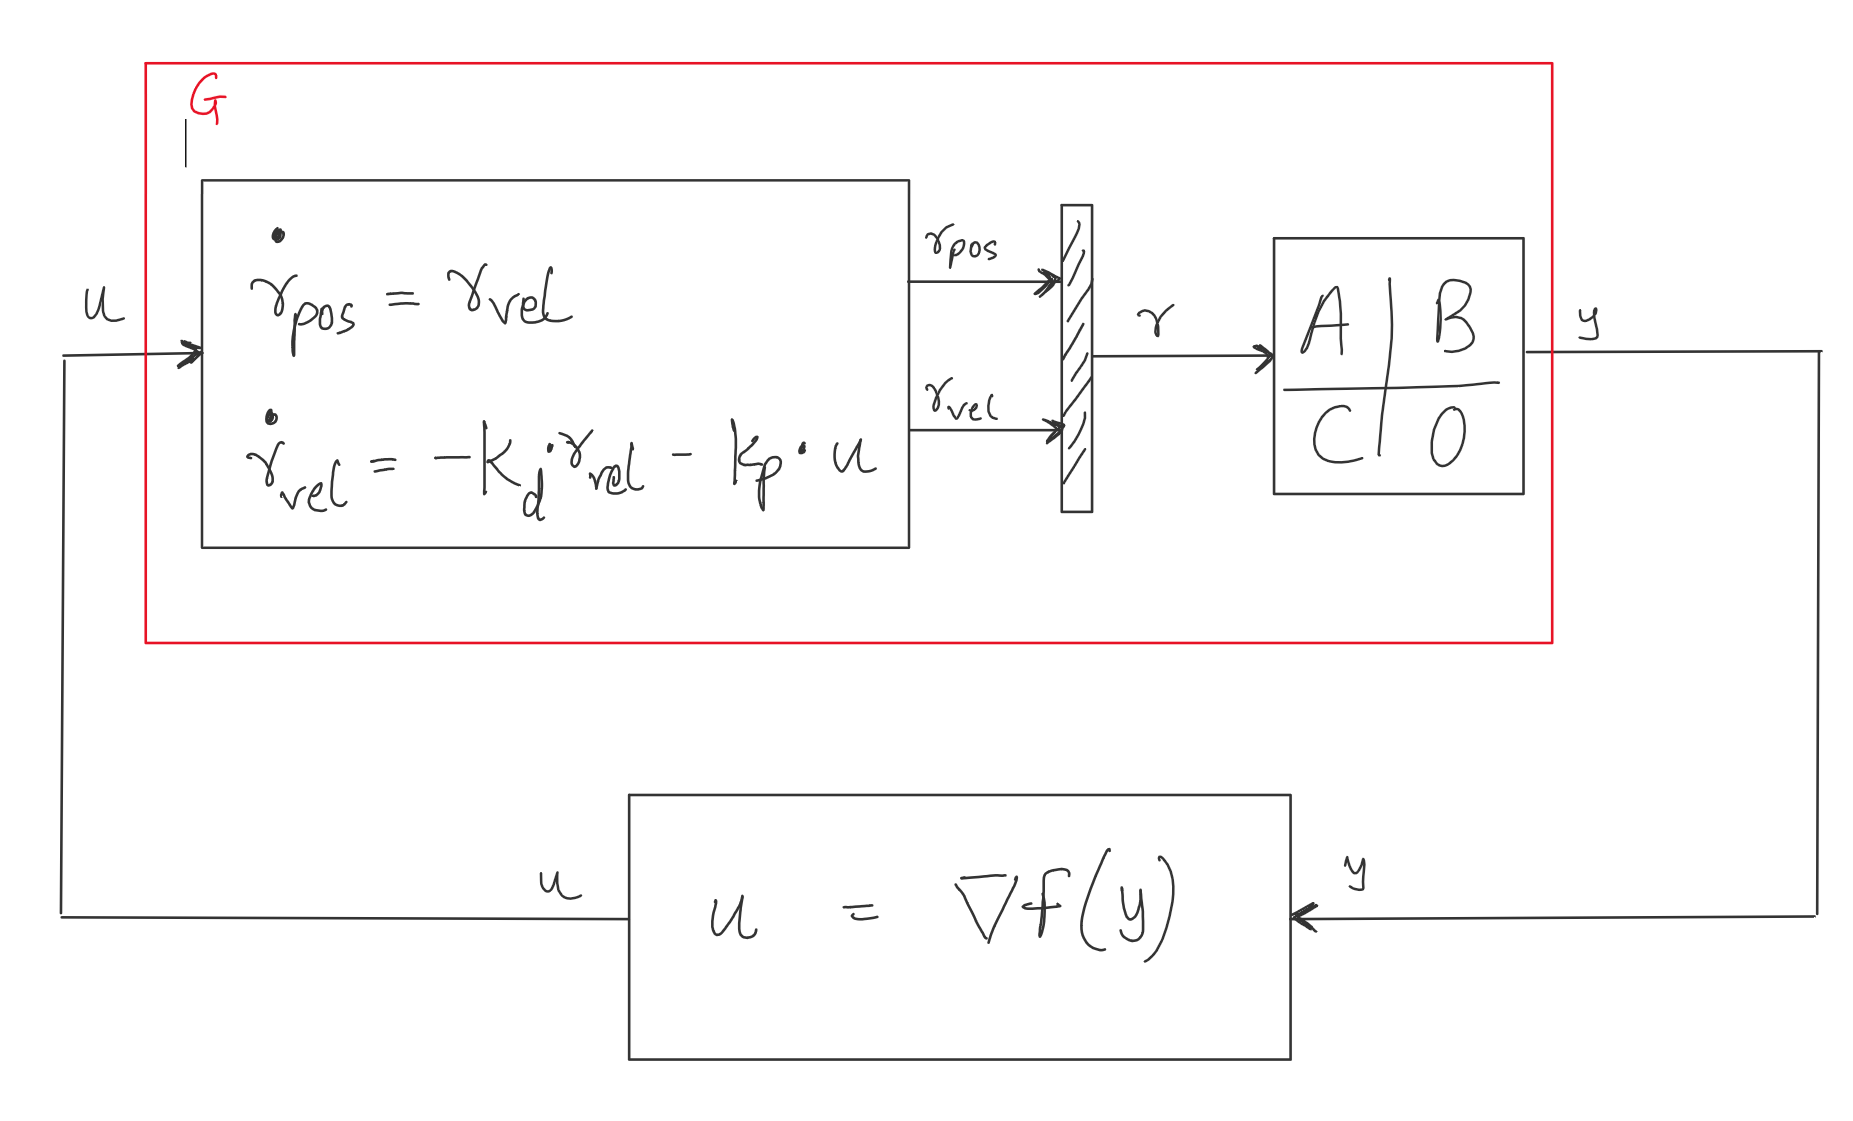
\includegraphics[width=8cm]{figures/Figure_IQC_paper.PNG}
		% This file was created by matlab2tikz.
%
%The latest updates can be retrieved from
%  http://www.mathworks.com/matlabcentral/fileexchange/22022-matlab2tikz-matlab2tikz
%where you can also make suggestions and rate matlab2tikz.
%
\definecolor{mycolor1}{rgb}{0.00000,1.00000,1.00000}%
%
\begin{tikzpicture}

\begin{axis}[%
width=2.321in,
height=2.266in,
at={(1in,2in)},
scale only axis,
xmin=1,
xmax=9,
xlabel style={font=\color{white!15!black}},
xlabel={$L$},
ymin=0,
ymax=0.5,
ylabel style={font=\color{white!15!black}},
ylabel={$\alpha$},
axis background/.style={fill=white},
title style={font=\bfseries},
title={},
legend style={legend cell align=left, align=left, draw=white!15!black}
]
\addplot [color=red]
  table[row sep=crcr]{%
1	0.4119873046875\\
1.1	0.3741455078125\\
1.2	0.3472900390625\\
1.3	0.325927734375\\
1.4	0.3076171875\\
1.5	0.291748046875\\
1.6	0.277099609375\\
1.7	0.263671875\\
1.8	0.2508544921875\\
1.9	0.2386474609375\\
2	0.2276611328125\\
2.1	0.2166748046875\\
2.2	0.2069091796875\\
2.3	0.1971435546875\\
2.4	0.1873779296875\\
2.5	0.17822265625\\
2.6	0.1690673828125\\
2.7	0.1605224609375\\
2.8	0.152587890625\\
2.9	0.14404296875\\
3	0.1361083984375\\
3.1	0.1287841796875\\
3.2	0.120849609375\\
3.3	0.113525390625\\
3.4	0.106201171875\\
3.5	0.0994873046875\\
3.6	0.0921630859375\\
3.7	0.08544921875\\
3.8	0.0787353515625\\
3.9	0.072021484375\\
4	0.06591796875\\
4.1	0.0592041015625\\
4.2	0.0531005859375\\
4.3	0.0469970703125\\
4.4	0.0408935546875\\
4.5	0.0347900390625\\
4.6	0.029296875\\
4.7	0.023193359375\\
4.8	0.0177001953125\\
4.9	0.01220703125\\
5	0.006103515625\\
5.1	0.0006103515625\\
5.2	-1\\
5.3	-1\\
5.4	-1\\
5.5	-1\\
5.6	-1\\
5.7	-1\\
5.8	-1\\
5.9	-1\\
6	-1\\
6.1	-1\\
6.2	-1\\
6.3	-1\\
6.4	-1\\
6.5	-1\\
6.6	-1\\
6.7	-1\\
6.8	-1\\
6.9	-1\\
7	-1\\
7.1	-1\\
7.2	-1\\
7.3	-1\\
7.4	-1\\
7.5	-1\\
7.6	-1\\
7.7	-1\\
7.8	-1\\
7.9	-1\\
8	-1\\
8.1	-1\\
8.2	-1\\
8.3	-1\\
8.4	-1\\
8.5	-1\\
8.6	-1\\
8.7	-1\\
8.8	-1\\
8.9	-1\\
9	-1\\
9.1	-1\\
9.2	-1\\
9.3	-1\\
9.4	-1\\
9.5	-1\\
9.6	-1\\
9.7	-1\\
9.8	-1\\
9.9	-1\\
10	-1\\
};
\addlegendentry{CC}

\addplot [color=green]
  table[row sep=crcr]{%
1	0.4119873046875\\
1.1	0.38330078125\\
1.2	0.3643798828125\\
1.3	0.350341796875\\
1.4	0.33935546875\\
1.5	0.32958984375\\
1.6	0.321044921875\\
1.7	0.313720703125\\
1.8	0.306396484375\\
1.9	0.30029296875\\
2	0.2935791015625\\
2.1	0.2880859375\\
2.2	0.281982421875\\
2.3	0.2764892578125\\
2.4	0.27099609375\\
2.5	0.2655029296875\\
2.6	0.260009765625\\
2.7	0.2545166015625\\
2.8	0.2490234375\\
2.9	0.2435302734375\\
3	0.2386474609375\\
3.1	0.233154296875\\
3.2	0.2276611328125\\
3.3	0.2227783203125\\
3.4	0.21728515625\\
3.5	0.2117919921875\\
3.6	0.2069091796875\\
3.7	0.201416015625\\
3.8	0.196533203125\\
3.9	0.1910400390625\\
4	0.1861572265625\\
4.1	0.1806640625\\
4.2	0.17578125\\
4.3	0.1708984375\\
4.4	0.1654052734375\\
4.5	0.1605224609375\\
4.6	0.1556396484375\\
4.7	0.150146484375\\
4.8	0.145263671875\\
4.9	0.140380859375\\
5	0.135498046875\\
5.1	0.130615234375\\
5.2	0.125732421875\\
5.3	0.120849609375\\
5.4	0.115966796875\\
5.5	0.111083984375\\
5.6	0.1068115234375\\
5.7	0.1019287109375\\
5.8	0.0970458984375\\
5.9	0.0927734375\\
6	0.087890625\\
6.1	0.0836181640625\\
6.2	0.0787353515625\\
6.3	0.074462890625\\
6.4	0.069580078125\\
6.5	0.0653076171875\\
6.6	0.06103515625\\
6.7	0.05615234375\\
6.8	0.0518798828125\\
6.9	0.047607421875\\
7	0.0433349609375\\
7.1	0.0390625\\
7.2	0.0347900390625\\
7.3	0.030517578125\\
7.4	0.0262451171875\\
7.5	0.02197265625\\
7.6	0.0177001953125\\
7.7	0.0140380859375\\
7.8	0.009765625\\
7.9	0.0054931640625\\
8	0.0018310546875\\
8.1	-1\\
8.2	-1\\
8.3	-1\\
8.4	-1\\
8.5	-1\\
8.6	-1\\
8.7	-1\\
8.8	-1\\
8.9	-1\\
9	-1\\
9.1	-1\\
9.2	-1\\
9.3	-1\\
9.4	-1\\
9.5	-1\\
9.6	-1\\
9.7	-1\\
9.8	-1\\
9.9	-1\\
10	-1\\
};
\addlegendentry{ZFb causal}

\addplot [color=blue, only marks, mark=o, mark options={solid, blue}]
  table[row sep=crcr]{%
1	0.4119873046875\\
1.1	0.3741455078125\\
1.2	0.3472900390625\\
1.3	0.325927734375\\
1.4	0.3076171875\\
1.5	0.291748046875\\
1.6	0.277099609375\\
1.7	0.263671875\\
1.8	0.2508544921875\\
1.9	0.2386474609375\\
2	0.2276611328125\\
2.1	0.2166748046875\\
2.2	0.2069091796875\\
2.3	0.1971435546875\\
2.4	0.1873779296875\\
2.5	0.17822265625\\
2.6	0.1690673828125\\
2.7	0.1605224609375\\
2.8	0.152587890625\\
2.9	0.14404296875\\
3	0.1361083984375\\
3.1	0.1287841796875\\
3.2	0.120849609375\\
3.3	0.113525390625\\
3.4	0.106201171875\\
3.5	0.0994873046875\\
3.6	0.0921630859375\\
3.7	0.08544921875\\
3.8	0.0787353515625\\
3.9	0.072021484375\\
4	0.06591796875\\
4.1	0.0592041015625\\
4.2	0.0531005859375\\
4.3	0.0469970703125\\
4.4	0.0408935546875\\
4.5	0.0347900390625\\
4.6	0.029296875\\
4.7	0.023193359375\\
4.8	0.0177001953125\\
4.9	0.01220703125\\
5	0.006103515625\\
5.1	0.0006103515625\\
5.2	-1\\
5.3	-1\\
5.4	-1\\
5.5	-1\\
5.6	-1\\
5.7	-1\\
5.8	-1\\
5.9	-1\\
6	-1\\
6.1	-1\\
6.2	-1\\
6.3	-1\\
6.4	-1\\
6.5	-1\\
6.6	-1\\
6.7	-1\\
6.8	-1\\
6.9	-1\\
7	-1\\
7.1	-1\\
7.2	-1\\
7.3	-1\\
7.4	-1\\
7.5	-1\\
7.6	-1\\
7.7	-1\\
7.8	-1\\
7.9	-1\\
8	-1\\
8.1	-1\\
8.2	-1\\
8.3	-1\\
8.4	-1\\
8.5	-1\\
8.6	-1\\
8.7	-1\\
8.8	-1\\
8.9	-1\\
9	-1\\
9.1	-1\\
9.2	-1\\
9.3	-1\\
9.4	-1\\
9.5	-1\\
9.6	-1\\
9.7	-1\\
9.8	-1\\
9.9	-1\\
10	-1\\
};
\addlegendentry{ZFb anti causal}

\addplot [color=mycolor1]
  table[row sep=crcr]{%
1	0.4119873046875\\
1.1	0.404052734375\\
1.2	0.3955078125\\
1.3	0.3875732421875\\
1.4	0.379638671875\\
1.5	0.3717041015625\\
1.6	0.3643798828125\\
1.7	0.3564453125\\
1.8	0.34912109375\\
1.9	0.3411865234375\\
2	0.3338623046875\\
2.1	0.3265380859375\\
2.2	0.3192138671875\\
2.3	0.3125\\
2.4	0.30517578125\\
2.5	0.2984619140625\\
2.6	0.2911376953125\\
2.7	0.284423828125\\
2.8	0.2777099609375\\
2.9	0.27099609375\\
3	0.2642822265625\\
3.1	0.2581787109375\\
3.2	0.25146484375\\
3.3	0.245361328125\\
3.4	0.2386474609375\\
3.5	0.2325439453125\\
3.6	0.2264404296875\\
3.7	0.2203369140625\\
3.8	0.2142333984375\\
3.9	0.2081298828125\\
4	0.20263671875\\
4.1	0.196533203125\\
4.2	0.1910400390625\\
4.3	0.1849365234375\\
4.4	0.179443359375\\
4.5	0.1739501953125\\
4.6	0.16845703125\\
4.7	0.1629638671875\\
4.8	0.157470703125\\
4.9	0.1519775390625\\
5	0.146484375\\
5.1	0.1409912109375\\
5.2	0.1361083984375\\
5.3	0.130615234375\\
5.4	0.125732421875\\
5.5	0.1202392578125\\
5.6	0.1153564453125\\
5.7	0.1104736328125\\
5.8	0.1055908203125\\
5.9	0.1007080078125\\
6	0.0958251953125\\
6.1	0.0909423828125\\
6.2	0.0860595703125\\
6.3	0.0811767578125\\
6.4	0.0762939453125\\
6.5	0.072021484375\\
6.6	0.067138671875\\
6.7	0.062255859375\\
6.8	0.0579833984375\\
6.9	0.0537109375\\
7	0.048828125\\
7.1	0.0445556640625\\
7.2	0.040283203125\\
7.3	0.035400390625\\
7.4	0.0311279296875\\
7.5	0.02685546875\\
7.6	0.0225830078125\\
7.7	0.018310546875\\
7.8	0.0140380859375\\
7.9	0.0103759765625\\
8	0.006103515625\\
8.1	0.0018310546875\\
8.2	-1\\
8.3	-1\\
8.4	-1\\
8.5	-1\\
8.6	-1\\
8.7	-1\\
8.8	-1\\
8.9	-1\\
9	-1\\
9.1	-1\\
9.2	-1\\
9.3	-1\\
9.4	-1\\
9.5	-1\\
9.6	-1\\
9.7	-1\\
9.8	-1\\
9.9	-1\\
10	-1\\
};
\addlegendentry{ZFb non causal}

\addplot [color=black, only marks, mark=o, mark options={solid, black}]
  table[row sep=crcr]{%
1	0.412331651029502\\
1.1	0.404104631075646\\
1.2	0.395974289263065\\
1.3	0.387939741864961\\
1.4	0.380000019452198\\
1.5	0.372154077971261\\
1.6	0.364400808966183\\
1.7	0.356739048974318\\
1.8	0.349167588131177\\
1.9	0.341685178023271\\
2	0.334290538830462\\
2.1	0.326982365800579\\
2.2	0.319759335099553\\
2.3	0.312620109080054\\
2.4	0.305563341010739\\
2.5	0.298587679307016\\
2.6	0.291691771302537\\
2.7	0.284874266598906\\
2.8	0.278133820029051\\
2.9	0.271469094267668\\
3	0.26487876212005\\
3.1	0.258361508518492\\
3.2	0.251916032253452\\
3.3	0.245541047464569\\
3.4	0.239235284914789\\
3.5	0.232997493068939\\
3.6	0.226826438996406\\
3.7	0.220720909115899\\
3.8	0.214679709798701\\
3.9	0.208701667845465\\
4	0.202785630850187\\
4.1	0.196930467463774\\
4.2	0.191135067568535\\
4.3	0.185398342373745\\
4.4	0.179719224441609\\
4.5	0.174096667651941\\
4.6	0.168529647113125\\
4.7	0.163017159026185\\
4.8	0.157558220508055\\
4.9	0.152151869379587\\
5	0.146797163923227\\
5.1	0.141493182614812\\
5.2	0.136239023833451\\
5.3	0.131033805553032\\
5.4	0.125876665018558\\
5.5	0.120766758410098\\
5.6	0.115703260496917\\
5.7	0.110685364283959\\
5.8	0.105712280652736\\
5.9	0.100783237998324\\
6	0.0958974818640143\\
6.1	0.091054274575032\\
6.2	0.0862528948724395\\
6.3	0.0814926375483512\\
6.4	0.0767728130832954\\
6.5	0.072092747286594\\
6.6	0.0674517809403497\\
6.7	0.062849269447712\\
6.8	0.0582845824858739\\
6.9	0.0537571036642326\\
7	0.0492662301880663\\
7.1	0.0448113725280309\\
7.2	0.0403919540956924\\
7.3	0.0360074109253169\\
7.4	0.0316571913620152\\
7.5	0.0273407557564156\\
7.6	0.0230575761658652\\
7.7	0.0188071360622775\\
7.8	0.0145889300465936\\
7.9	0.0104024635698768\\
8	0.00624725266099616\\
8.1	0.00212282366089683\\
8.2	-0.00197128703662988\\
8.3	-0.00603553323776879\\
8.4	-0.0100703591950907\\
8.5	-0.0140761998477345\\
8.6	-0.0180534810554153\\
8.7	-0.0220026198263578\\
8.8	-0.0259240245392573\\
8.9	-0.0298180951594347\\
9	-0.0336852234492339\\
9.1	-0.0375257931728344\\
9.2	-0.0413401802955638\\
9.3	-0.0451287531778723\\
9.4	-0.0488918727640491\\
9.5	-0.0526298927658563\\
9.6	-0.0563431598411483\\
9.7	-0.0600320137676526\\
9.8	-0.0636967876120013\\
9.9	-0.0673378078941474\\
10	-0.0709553947472893\\
};
\addlegendentry{Example field}

\end{axis}

\begin{axis}[%
width=5.833in,
height=4.375in,
at={(0in,0in)},
scale only axis,
xmin=0,
xmax=1,
ymin=0,
ymax=1,
axis line style={draw=none},
ticks=none,
axis x line*=bottom,
axis y line*=left
]
\end{axis}
\end{tikzpicture}%
		\caption{Robustness for Quadrotor and $m=1$}
		\centering
		\label{fig:quadrotor_robustness}
	\end{figure}
\end{frame}
%%%%%%%%%%%%%%%%%%%%%%%%%%%%%%%%%%%%%%%%%%%%%%%%%%%%%%%%%%%%%%%%%%%%%%
%\begin{frame}{Tuning $kp,kd$ for a single quadrotor}
%	\begin{figure}[t]
%		%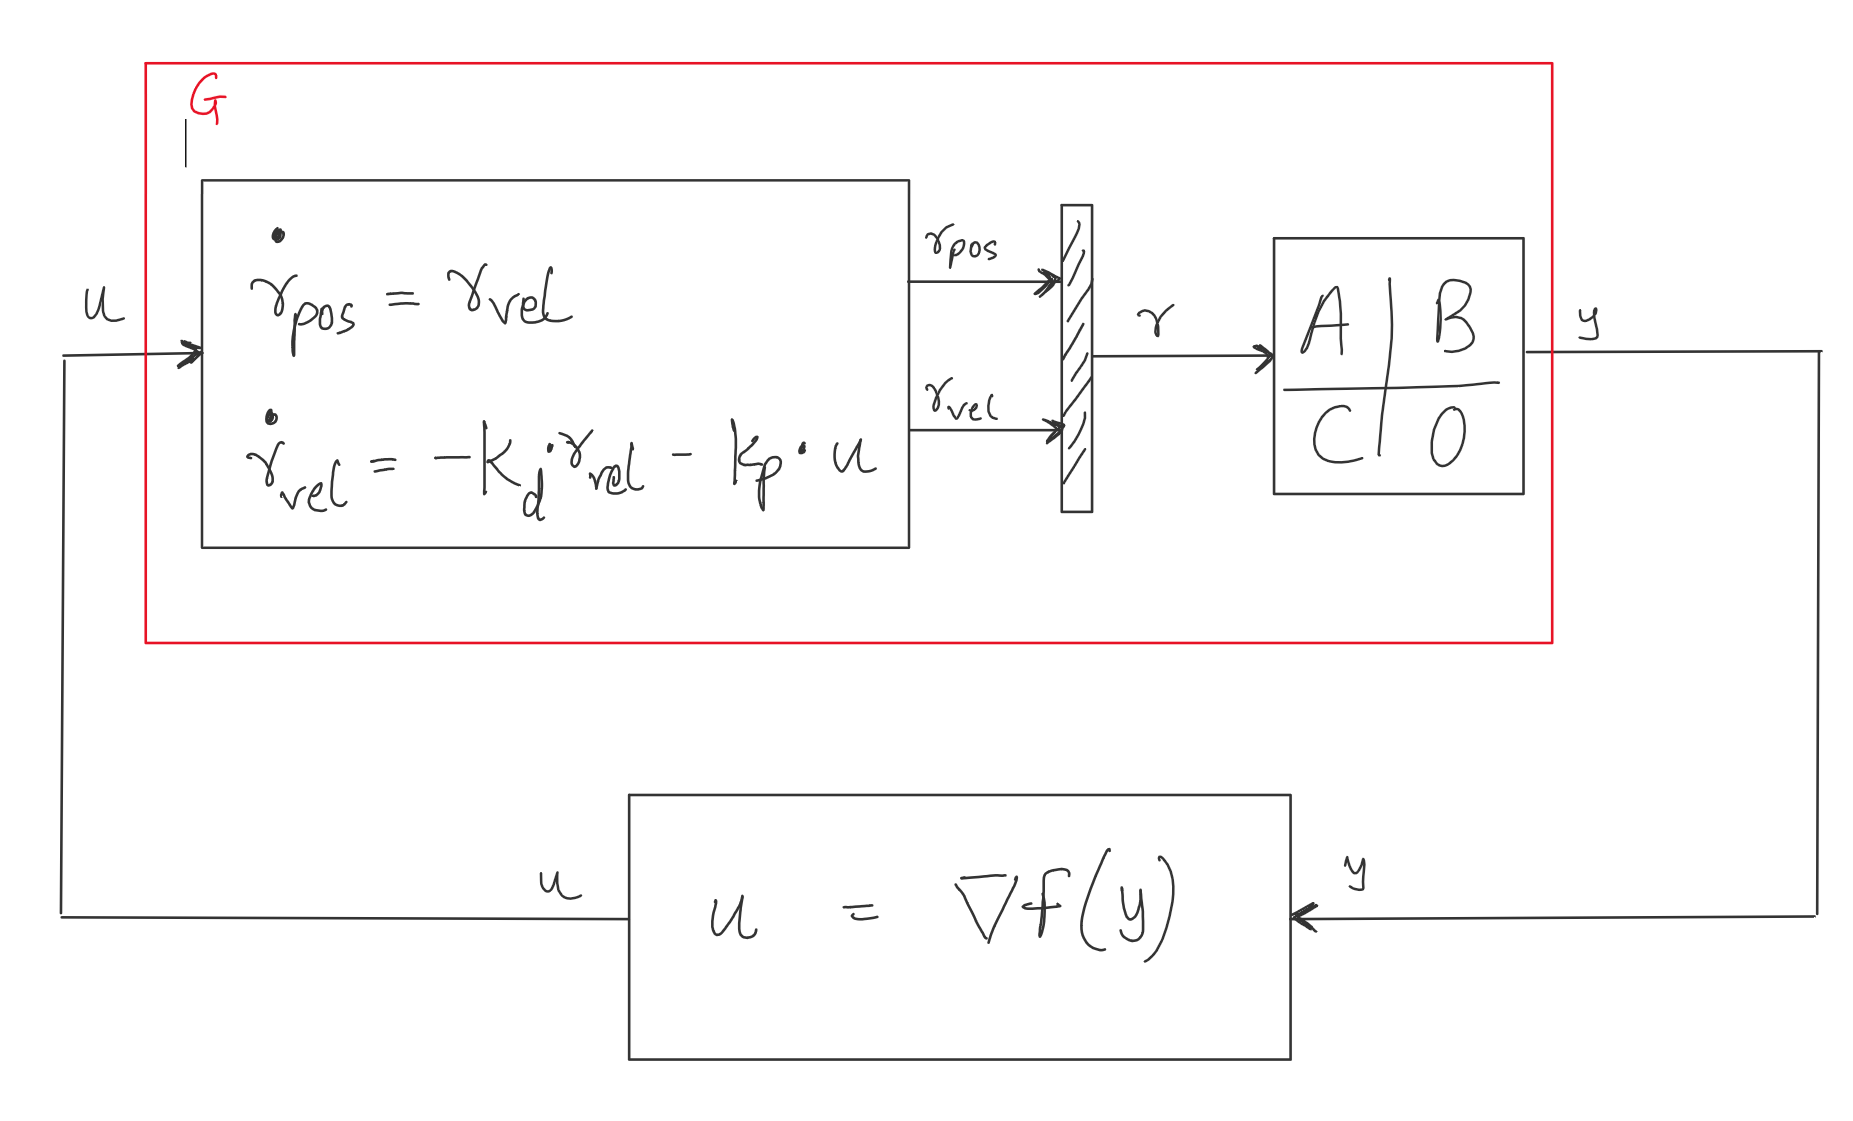
\includegraphics[width=8cm]{figures/Figure_IQC_paper.PNG}
%		% This file was created by matlab2tikz.
%
%The latest updates can be retrieved from
%  http://www.mathworks.com/matlabcentral/fileexchange/22022-matlab2tikz-matlab2tikz
%where you can also make suggestions and rate matlab2tikz.
%
\definecolor{mycolor1}{rgb}{0.00000,0.44700,0.74100}%
\definecolor{mycolor2}{rgb}{0.85000,0.32500,0.09800}%
%
\begin{tikzpicture}

\begin{axis}[%
width=2.321in,
height=2.266in,
at={(1in,2in)},
scale only axis,
xmin=5,
xmax=20,
xlabel style={font=\color{white!15!black}},
xlabel={$\frac{k_d}{k_p}$},
ymin=0,
ymax=0.2,
ylabel style={font=\color{white!15!black}},
ylabel={$\alpha$},
axis background/.style={fill=white},
title style={font=\bfseries},
title={},
legend style={legend cell align=left, align=left, draw=white!15!black}
]
\addplot [color=mycolor1, only marks, mark=asterisk, mark options={solid, mycolor1}]
  table[row sep=crcr]{%
0.2	-1\\
0.6	-1\\
1	-1\\
1.4	-1\\
1.8	-1\\
2.2	-1\\
2.6	-1\\
3	-1\\
3.4	-1\\
3.8	-1\\
4.2	-1\\
4.6	-1\\
5	-1\\
5.4	-1\\
5.8	-1\\
6.2	-1\\
6.6	-1\\
7	-1\\
7.4	-1\\
7.8	-1\\
8.2	-1\\
8.6	-1\\
9	-1\\
9.4	-1\\
9.8	-1\\
10.2	0.001220703125\\
10.6	0.008544921875\\
11	0.0152587890625\\
11.4	0.0213623046875\\
11.8	0.0262451171875\\
12.2	0.03173828125\\
12.6	0.0360107421875\\
13	0.040283203125\\
13.4	0.0439453125\\
13.8	0.0469970703125\\
14.2	0.050048828125\\
14.6	0.052490234375\\
15	0.054931640625\\
15.4	0.0567626953125\\
15.8	0.0579833984375\\
16.2	0.0592041015625\\
16.6	0.059814453125\\
17	0.0604248046875\\
17.4	0.0604248046875\\
17.8	0.0604248046875\\
18.2	0.059814453125\\
18.6	0.05859375\\
19	0.057373046875\\
19.4	0.05615234375\\
19.8	0.054931640625\\
};
\addlegendentry{CC}

\addplot [color=mycolor2, only marks, mark=asterisk, mark options={solid, mycolor2}]
  table[row sep=crcr]{%
0.2	-1\\
0.6	-1\\
1	-1\\
1.4	-1\\
1.8	-1\\
2.2	-1\\
2.6	-1\\
3	-1\\
3.4	-1\\
3.8	-1\\
4.2	-1\\
4.6	-1\\
5	-1\\
5.4	0.0164794921875\\
5.8	0.0408935546875\\
6.2	0.0628662109375\\
6.6	0.0830078125\\
7	0.101318359375\\
7.4	0.118408203125\\
7.8	0.13427734375\\
8.2	0.1483154296875\\
8.6	0.147705078125\\
9	0.13916015625\\
9.4	0.1312255859375\\
9.8	0.12451171875\\
10.2	0.118408203125\\
10.6	0.1129150390625\\
11	0.1080322265625\\
11.4	0.1031494140625\\
11.8	0.098876953125\\
12.2	0.09521484375\\
12.6	0.091552734375\\
13	0.0885009765625\\
13.4	0.08544921875\\
13.8	0.0823974609375\\
14.2	0.079345703125\\
14.6	0.076904296875\\
15	0.074462890625\\
15.4	0.0726318359375\\
15.8	0.0701904296875\\
16.2	0.068359375\\
16.6	0.0665283203125\\
17	0.064697265625\\
17.4	0.0634765625\\
17.8	0.0616455078125\\
18.2	0.059814453125\\
18.6	0.05859375\\
19	0.057373046875\\
19.4	0.05615234375\\
19.8	0.054931640625\\
};
\addlegendentry{ZFb}

\end{axis}

\begin{axis}[%
width=5.833in,
height=4.375in,
at={(0in,0in)},
scale only axis,
xmin=0,
xmax=1,
ymin=0,
ymax=1,
axis line style={draw=none},
ticks=none,
axis x line*=bottom,
axis y line*=left
]
\end{axis}
\end{tikzpicture}%
%		\caption{Robustness for Quadrotor and $m=1$}
%		\centering
%		\label{fig:optimal_kd_kp_ratio}
%	\end{figure}
%\end{frame}
%%%%%%%%%%%%%%%%%%%%%%%%%%%%%%%%%%%%%%%%%%%%%%%%%%%%%%%%%%%%%%%%%%%%%
%\begin{frame}{Quadrotor trajectory with a single quadrotor}	
%	Change the Figure
%	\begin{figure}[t]
%		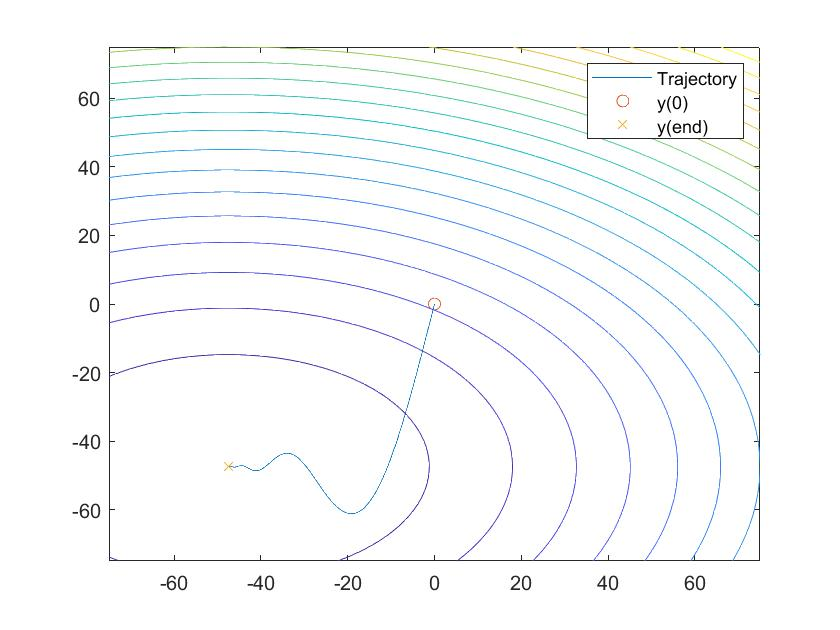
\includegraphics[width=8cm]{figures/quadrotor_trajectory.JPG}
%		%\input{figures/quadrotor_trajectory}
%		\caption{Robustness for Quadrotor and $m=1$}
%		\centering
%		\label{fig:quadrotor_trajectory}
%	\end{figure}
%\end{frame}
%%%%%%%%%%%%%%%%%%%%%%%%%%%%%%%%%%%%%%%%%%%%%%%%%%%%%%%%%%%%%%%%%%%%%
\section{Extension: Multiple agents}
%%%%%%%%%%%%%%%%%%%%%%%%%%%%%%%%%%%%%%%%%%%%%%%%%%%%%%%%%%%%%%%%%%%%%
\begin{frame}{Control Architecture: Multiple agents}
	\begin{equation*} %\label{eq:sys_dyn_G}
		\begin{split}
			\Dot{\hat{\eta}}(t)&=\hat{A}_G\hat{\eta}(t) + \hat{B}_G \hat{u}(t), \quad \quad \hat{\eta}(0)=\hat{\eta}_{0},\\
			\hat{y}(t)&=\hat{C}_G \hat{\eta}(t). \\
		\end{split}
	\end{equation*}
where, notation $\hat{X}=I_N \otimes X$ and $\hat{x}=[x_1^T,\hdots,x_N^T]^T$ is used.
\pause
\begin{block}{Formation control law with gradient-based forcing term}
\begin{equation}\label{eq:control_law}
	\hat{u}=\mathcal{L}_{(d)}(\hat{y}-\hat{r})+\begin{bmatrix}u_{\psi_1}\\ \vdots \\u_{\psi_N}\end{bmatrix}.
\end{equation}

\begin{equation}\label{eq:forcing_term}
	\begin{split}
		u_{\psi_i}(t)&=
		\begin{cases}
			\nabla \psi(y_i), & \text{if}\ i\in \mathcal{V}_l, \\
			0, & \text{otherwise}.
		\end{cases}
	\end{split}
\end{equation}
\end{block}
\end{frame}
%%%%%%%%%%%%%%%%%%%%%%%%%%%%%%%%%%%%%%%%%%%%%%%%%%%%%%%%%%%%%%%%%%%%%
\begin{frame}{Control Architecture: Multiple agents}
\begin{figure}[ht]
	\tikzstyle{block} = [draw, rectangle, 
    minimum height=3em, minimum width=6em]
\tikzstyle{sum} = [draw,  circle, node distance=1cm]
\tikzstyle{input} = [coordinate]
\tikzstyle{output} = [coordinate]
\tikzstyle{pinstyle} = [pin edge={to-,thin,black}]

% The block diagram code is probably more verbose than necessary
%\begin{tikzpicture}[auto, node distance=2cm,>=latex']
%    % We start by placing the blocks
%    \node [input, name=input] {};
%    \node [sum, right of=input] (sum) {};
%    \node [block, right of=sum] (controller) {Controller};
%    \node [block, right of=controller, pin={[pinstyle]above:Disturbances},
%            node distance=3cm] (system) {System};
%    % We draw an edge between the controller and system block to 
%    % calculate the coordinate u. We need it to place the measurement block. 
%    \draw [->] (controller) -- node[name=u] {$u$} (system);
%    \node [output, right of=system] (output) {};
%    \node [block, below of=u] (measurements) {Measurements};
%
%    % Once the nodes are placed, connecting them is easy. 
%    \draw [draw,->] (input) -- node {$r$} (sum);
%    \draw [->] (sum) -- node {$e$} (controller);
%    \draw [->] (system) -- node [name=y] {$y$}(output);
%    \draw [->] (y) |- (measurements);
%    \draw [->] (measurements) -| node[pos=0.99] {$-$} 
%        node [near end] {$y_m$} (sum);
%\end{tikzpicture}

\begin{tikzpicture}[auto, node distance=2cm,>=latex']
% We start by placing the blocks
\node [input, name=input] {};
\node [sum,right of=input](sum_ref) {};
\node [block, right of=input,node distance=3cm](L) {$\mathcal{L}\otimes I_d$};
\node [sum, right of=L,node distance=2cm](sum) {};
\node [block, right of=sum,node distance=2cm,minimum height=2.5em,minimum width=3em](G) {$\left[\begin{array}{c|c}
\hat{A}_G     &  \hat{B}_G\\
\hline
\hat{C}_G     &  \mathbf{0}
\end{array}\right]$};
\node [output, right of=G,node distance=2cm](output) {};
\node [output, right of=G,node distance=1.4cm](outmid) {};
\node [block, above of=G,node distance=2cm](u_psi) {$\begin{bmatrix}0\\ \nabla \psi(y_i)\\ 0\\ \vdots \end{bmatrix}$};
\node [output, below of=L,node distance=2cm](delta) {};


% Once the nodes are placed, connecting them is easy. 
\draw [draw,->] (input) -- node {$-\hat{r}$} (sum_ref);
\draw [draw,->] (sum_ref) -- (L);
\draw [draw,->] (L) -- (sum);
\draw [draw,->] (u_psi) -| (sum);
\draw [draw,->] (sum) -- node {$\hat{u}$} (G);
\draw [draw,->] (G) -- node{$\hat{y}$} (output);
\draw [-] (outmid) |- (delta);
\draw [->] (outmid) |- (u_psi);
\draw [->] (delta) -| (sum_ref);
\end{tikzpicture}
	\caption{Control architecture}
	%\label{fig:control_architecture}	
\end{figure}
%	\begin{equation} \label{eq:sys_dyn_G}
%		\begin{split}
%			\Dot{\hat{\eta}}(t)&=\hat{A}_G\hat{\eta}(t) + \hat{B}_G \hat{u}(t), \quad \quad \hat{\eta}(0)=\hat{\eta}_{0},\\
%			\hat{y}(t)&=\hat{C}_G \hat{\eta}(t). \\
%			\hat{u}(t)&=\mathcal{L}_{(d)}(\hat{y}-\hat{r})+\begin{bmatrix}0\\ \vdots \\ \nabla \psi(y_i)\\ \vdots \\ 0 \end{bmatrix} \leftarrow \textnormal{ if } i\in \mathcal{V}_l 
%		\end{split}
%	\end{equation}
\end{frame}
%%%%%%%%%%%%%%%%%%%%%%%%%%%%%%%%%%%%%%%%%%%%%%%%%%%%%%%%%%%%%%%%%%%%%
\begin{frame}{Formulation as a robust control problem}
	\begin{block}{Definition}	
		For a given graph $\mathcal{G}$ of order $N$ (with its corresponding laplacian $\mathcal{L}$), the leader set $\mathcal{V}_l$, a scalar field $\psi$ and a given formation reference vector $\hat{r} \in \mathbb{R}^{Nd}$, define a function $f:\mathbb{R}^{Nd}\rightarrow \mathbb{R}$ by
		\begin{equation}\label{eq:defn_f}
			f(\hat{y})=\frac{1}{2}(\hat{y}-\hat{r})^T\mathcal{L}_{(d)}(\hat{y}-\hat{r}) + \sum_{v_i \in \mathcal{V}_l} \psi(y_i).
		\end{equation}	
	\end{block}
	\pause
	\begin{block}{Overall close-loop system}
	\begin{equation} \label{eq:sys_dyn_G_hat}
		\begin{split}
			\Dot{\hat{\eta}}(t)&=\hat{A}_G\hat{\eta}(t) + \hat{B}_G \hat{u}(t), \quad \quad \hat{\eta}(0)=\hat{\eta}_{0},\\
			\hat{y}(t)&=\hat{C}_G \hat{\eta}(t), \\
			\hat{u}(t)&=\nabla f (\hat{y}(t)).
		\end{split}
	\end{equation}
	\end{block}
\end{frame}
%%%%%%%%%%%%%%%%%%%%%%%%%%%%%%%%%%%%%%%%%%%%%%%%%%%%%%%%%%%%%%%%%%%%%
\begin{frame}{Recall Theorem 1}
	\begin{equation*}
	\begin{split}
		\left[\begin{array}{c|c}
			\mathcal{A}     &  \mathcal{B}\\
			\hline
			\mathcal{C}     &  \mathcal{D}
		\end{array}\right]&=
		(\Pi \otimes I_N)\begin{bmatrix}
			\hat{G}\\
			I_{Nd}
		\end{bmatrix}
		=
		\left[
		\begin{array}{c|c}
			A_{\Pi} \otimes I_{N} & B_{\Pi} \otimes I_{N} \\
			\hline
			C_{\Pi} \otimes I_{N} & D_{\Pi} \otimes I_{N}
		\end{array}
		\right]\left[\begin{array}{c|c}
			\hat{A}_G     &  \hat{B}_G\\
			\hline		
			\hat{C}_G     &  \mathbf{0} \\
			\mathbf{0}     			&  I_{Nd}
		\end{array}\right]
	\end{split}
	\end{equation*}
\pause 
\begin{block}{Theorem 1 applied to the overall networked system}
	If $f\in \mathcal{S}(m,L)$, $y_*$ minimizes $f$ and $\exists \mathcal{X}>0,P \in \mathbb{P}$ such that
	\begin{equation*}%\label{eq:perf_LMI}
		\begin{bmatrix}
			\mathcal{A}^T\mathcal{X}+\mathcal{X}\mathcal{A}+2\alpha \mathcal{X}  & \mathcal{X}\mathcal{B} \\
			\mathcal{B}^T\mathcal{X}    & \mathbf{0}
		\end{bmatrix}
		+
		\begin{bmatrix}
			\mathcal{C}^T \\
			\mathcal{D}^T 
		\end{bmatrix}
		( P\otimes I_{Nd})
		\begin{bmatrix}
			\mathcal{C} & \mathcal{D} 
		\end{bmatrix}
		\leq 
		0,
	\end{equation*}
	then, $||y(t)-y_*(t)||\leq \kappa e^{-\alpha t}$ holds for all $t\geq 0$
\end{block}
\pause 
\begin{block}{Questions}
\begin{itemize}
	\item[1] How to characterize minimizers of $f$?
	\item[2] How to verify if $f\in \mathcal{S}(m,L)$?
	\item[3] Can we exploit this structure in the LMIs?   
\end{itemize}
\end{block}
\end{frame}
%%%%%%%%%%%%%%%%%%%%%%%%%%%%%%%%%%%%%%%%%%%%%%%%%%%%%%%%%%%%%%%%%%%%%
\begin{frame}{1. Minimizers of $f$}
	\begin{block}{Recall definiteion of $f$}
		$$f(\hat{y})=\frac{1}{2}(\hat{y}-\hat{r})^T\mathcal{L}_{(d)}(\hat{y}-\hat{r}) + \sum_{v_i \in \mathcal{V}_l} \psi(y_i).$$		
	\end{block}
	\pause
	\begin{block}{Assumptions}
	\begin{itemize}
		\item[1] Let $\psi \in \mathcal{S}(m_{\psi},L_{\psi})$ for some $0<m_{\psi}\leq L_{\psi}$ and let $y_*$ minimize $\psi$.
		\item[2] For every node $v_i \in \mathcal{V}$, there is a node $v_j \in \mathcal{V}_l$ such that $\mathcal{G}$ contains an $i-j$ path.
	\end{itemize}
	\end{block}
\pause 
\begin{block}{Separately consider the cases}
\begin{itemize} 
	\item[1] Consensus $\hat{r}=\mathbf{0},|\mathcal{V}_l|\geq 1$
	\item[2] Formation control with single leader $\hat{r}\neq \mathbf{0}$, $|\mathcal{V}_l|=1$
	\item[3] Formation control with multiple leaders $\hat{r}\neq \mathbf{0}$, $|\mathcal{V}_l|>1$
\end{itemize}
\end{block}
\end{frame}
%%%%%%%%%%%%%%%%%%%%%%%%%%%%%%%%%%%%%%%%%%%%%%%%%%%%%%%%%%%%%%%%%%%%%
\begin{frame}{1. Minimizers of $f$}
	\begin{block}{Recall definiteion of $f$}
		$$f(\hat{y})=\frac{1}{2}(\hat{y}-\hat{r})^T\mathcal{L}_{(d)}(\hat{y}-\hat{r}) + \sum_{v_i \in \mathcal{V}_l} \psi(y_i).$$		
	\end{block}
	\begin{block}{Lemma (Consensus)}
	Let Assumptions 1 and 2 hold and let $\hat{r}=0$.
	Then, $\hat{y}$ is the minimizer of $f$ iff $\hat{y}=\mathbf{1}_N \otimes y_*$.
	\end{block}
\pause 
\begin{block}{Lemma(Formation with one leader)}
	Let Assumptions 1 and 2 hold and let $|\mathcal{V}_l|=1$.
	Then, $\hat{y}$ is the minimizer of $f$ iff $\hat{y}_i=y_*$ for $i \in \mathcal{V}_l$ and $y_j=y_*+(r_j-r_i)$ for all $j \in \mathcal{V}$.
\end{block}
\pause 
\begin{block}{Conjecture (Formation with multiple leaders)}
	Let Assumptions 1 and 2 hold. 
	The unique minimizer $y_*$ of $\psi$ lies in the convex hull of positions of leader agents. 
	%Furthermore, for quadratic fields, the average positions of the leaders coincides with $y_*$.
\end{block}
\end{frame}
%%%%%%%%%%%%%%%%%%%%%%%%%%%%%%%%%%%%%%%%%%%%%%%%%%%%%%%%%%%%%%%%%%%%%
\begin{frame}{2. Smoothness and convexity of $f$}
\begin{block}{Definition of grounded Laplacians}
	Define grounded Laplacians
	\begin{equation} \label{eq:Lgs_defn}
		\begin{split}
			\mathcal{L}_s&=\mathcal{L}+m_{\psi} E, \\
			\mathcal{L}_b&=\mathcal{L}+L_{\psi} E, \\
		\end{split}
	\end{equation}
	where, $E$ is a diagonal matrix with the $i^{th}$ diagonal entry equal to $1$ if $i \in \mathcal{V}_l$ and equal to $0$ otherwise.
\end{block}
\pause 
\begin{block}{Lemma}
	For constants $0<m \leq L$, the following two statements are equivalent:
\begin{enumerate}
	\item $f\in \mathcal{S}(m,L) \textnormal{ for all } \psi \in \mathcal{S}(m_{\psi},L_{\psi})$,
	\item $m I_N \preceq  \mathcal{L}_b \preceq \mathcal{L}_s \preceq L I_N$
\end{enumerate}
\end{block}
\end{frame}
%%%%%%%%%%%%%%%%%%%%%%%%%%%%%%%%%%%%%%%%%%%%%%%%%%%%%%%%%%%%%%%%%%%%%
\begin{frame}{3. Decomposition}
	\begin{block}{Define}
		$\left[\begin{array}{c|c}
			\mathcal{A}     &  \mathcal{B}\\
			\hline
			\mathcal{C}     &  \mathcal{D}
		\end{array}\right]=
		(\Pi \otimes I_N)\begin{bmatrix}
			\hat{G}\\
			I_{Nd}
		\end{bmatrix}$ and $
		\left[\begin{array}{c|c}
			\mathcal{A}_0     &  \mathcal{B}_0\\
			\hline
			\mathcal{C}_0     &  \mathcal{D}_0
		\end{array}\right]=
		\Pi\begin{bmatrix}
			G\\
			I_{d}
		\end{bmatrix}$
	\end{block}
		\pause 
		\begin{equation}\label{eq:perf_LMI}
				\begin{bmatrix}
					\mathcal{A}^T\mathcal{X}+\mathcal{X}\mathcal{A}+2\alpha \mathcal{X}  & \mathcal{X}\mathcal{B} \\
					\mathcal{B}^T\mathcal{X}    & \mathbf{0}
				\end{bmatrix}
				+
				(*)
				( P\otimes I_{Nd})
				\begin{bmatrix}
					\mathcal{C} & \mathcal{D} 
				\end{bmatrix}
				\leq 
				0,
			\end{equation}	
		\begin{equation}\label{eq:perf_LMI_small}
			\begin{bmatrix}
				\mathcal{A}_0^T\mathcal{X}_0+\mathcal{X}_0\mathcal{A}_0+2\alpha \mathcal{X}_0  & \mathcal{X}_0\mathcal{B}_0 \\
				\mathcal{B}_0^T\mathcal{X}_0    & \mathbf{0}
			\end{bmatrix}
			+
			(*)
			( P\otimes I_{d})
			\begin{bmatrix}
				\mathcal{C}_0 & \mathcal{D}_0 
			\end{bmatrix}
			\leq 
			0,
		\end{equation}
	\pause 
	\begin{block}{Theorem}
	The following statements are equivalent:
	\begin{enumerate}
		\item $\exists \mathcal{X}>0,P \in \mathbb{P}$ such that \eqref{eq:perf_LMI} is satisfied.
		\item $\exists \mathcal{X}_0>0,P \in \mathbb{P}$ such that \eqref{eq:perf_LMI_small} is satisfied.
	\end{enumerate}	
	\end{block}
\end{frame}
%%%%%%%%%%%%%%%%%%%%%%%%%%%%%%%%%%%%%%%%%%%%%%%%%%%%%%%%%%%%%%%%%%%%%
\begin{frame}{Final Analysis result}
	\begin{block}{Definition}
	\begin{equation}
		\begin{split}
		\Delta_{m,L}&=\{(\mathcal{G},\mathcal{V}_l,\psi):\psi \in \mathcal{S}(m_{\psi},L_{\psi}),f \in \mathcal{S}(m,L) \}\\
			&=\{(\mathcal{G},\mathcal{V}_l,\psi):\psi \in \mathcal{S}(m_{\psi},L_{\psi}),m I_N \preceq  \mathcal{L}_b \preceq \mathcal{L}_s \preceq L I_N \}
		\end{split}		
	\end{equation}
	\end{block}
\pause 
\begin{theorem}
	Let $(\mathcal{G},\mathcal{V}_l,\psi) \in \Delta_{m,L}$ for some $0<m\leq L$.
	If $\exists \mathcal{X}_0>0,P \in \mathbb{P}$ such that 
	\begin{equation}%\label{eq:perf_LMI_small}
		\begin{bmatrix}
			\mathcal{A}_0^T\mathcal{X}_0+\mathcal{X}_0\mathcal{A}_0+2\alpha \mathcal{X}_0  & \mathcal{X}_0\mathcal{B}_0 \\
			\mathcal{B}_0^T\mathcal{X}_0    & \mathbf{0}
		\end{bmatrix}
		+
		(*)
		( P\otimes I_{d})
		\begin{bmatrix}
			\mathcal{C}_0 & \mathcal{D}_0 
		\end{bmatrix}
		\leq 
		0,
	\end{equation} is satisfied, then, $||y(t)-y_*(t)||\leq \kappa e^{-\alpha t}$ holds for all $t\geq 0$.
\end{theorem}
\end{frame}
%%%%%%%%%%%%%%%%%%%%%%%%%%%%%%%%%%%%%%%%%%%%%%%%%%%%%%%%%%%%%%%%%%%%%
\section{Numerical results}
%%%%%%%%%%%%%%%%%%%%%%%%%%%%%%%%%%%%%%%%%%%%%%%%%%%%%%%%%%%%%%%%%%%%%
\begin{frame}{Example 1: Conservatism}
$\Delta_1 = \{(\mathcal{G},\mathcal{V}_l,\psi):\mathcal{G}=\mathcal{G}_{\textnormal{star}}^5,\mathcal{V}_l=\{1\} , \psi \in \mathcal{S}(2.02,L_{\psi})\} \subset \Delta_{0.3,L}$

$\Delta_2 = \{(\mathcal{G}^{25},\mathcal{V}_l,\psi):\psi = 1.85 ||y-y_*||^2 \} \subset \Delta_{m,L}$
\begin{figure}[t]
	%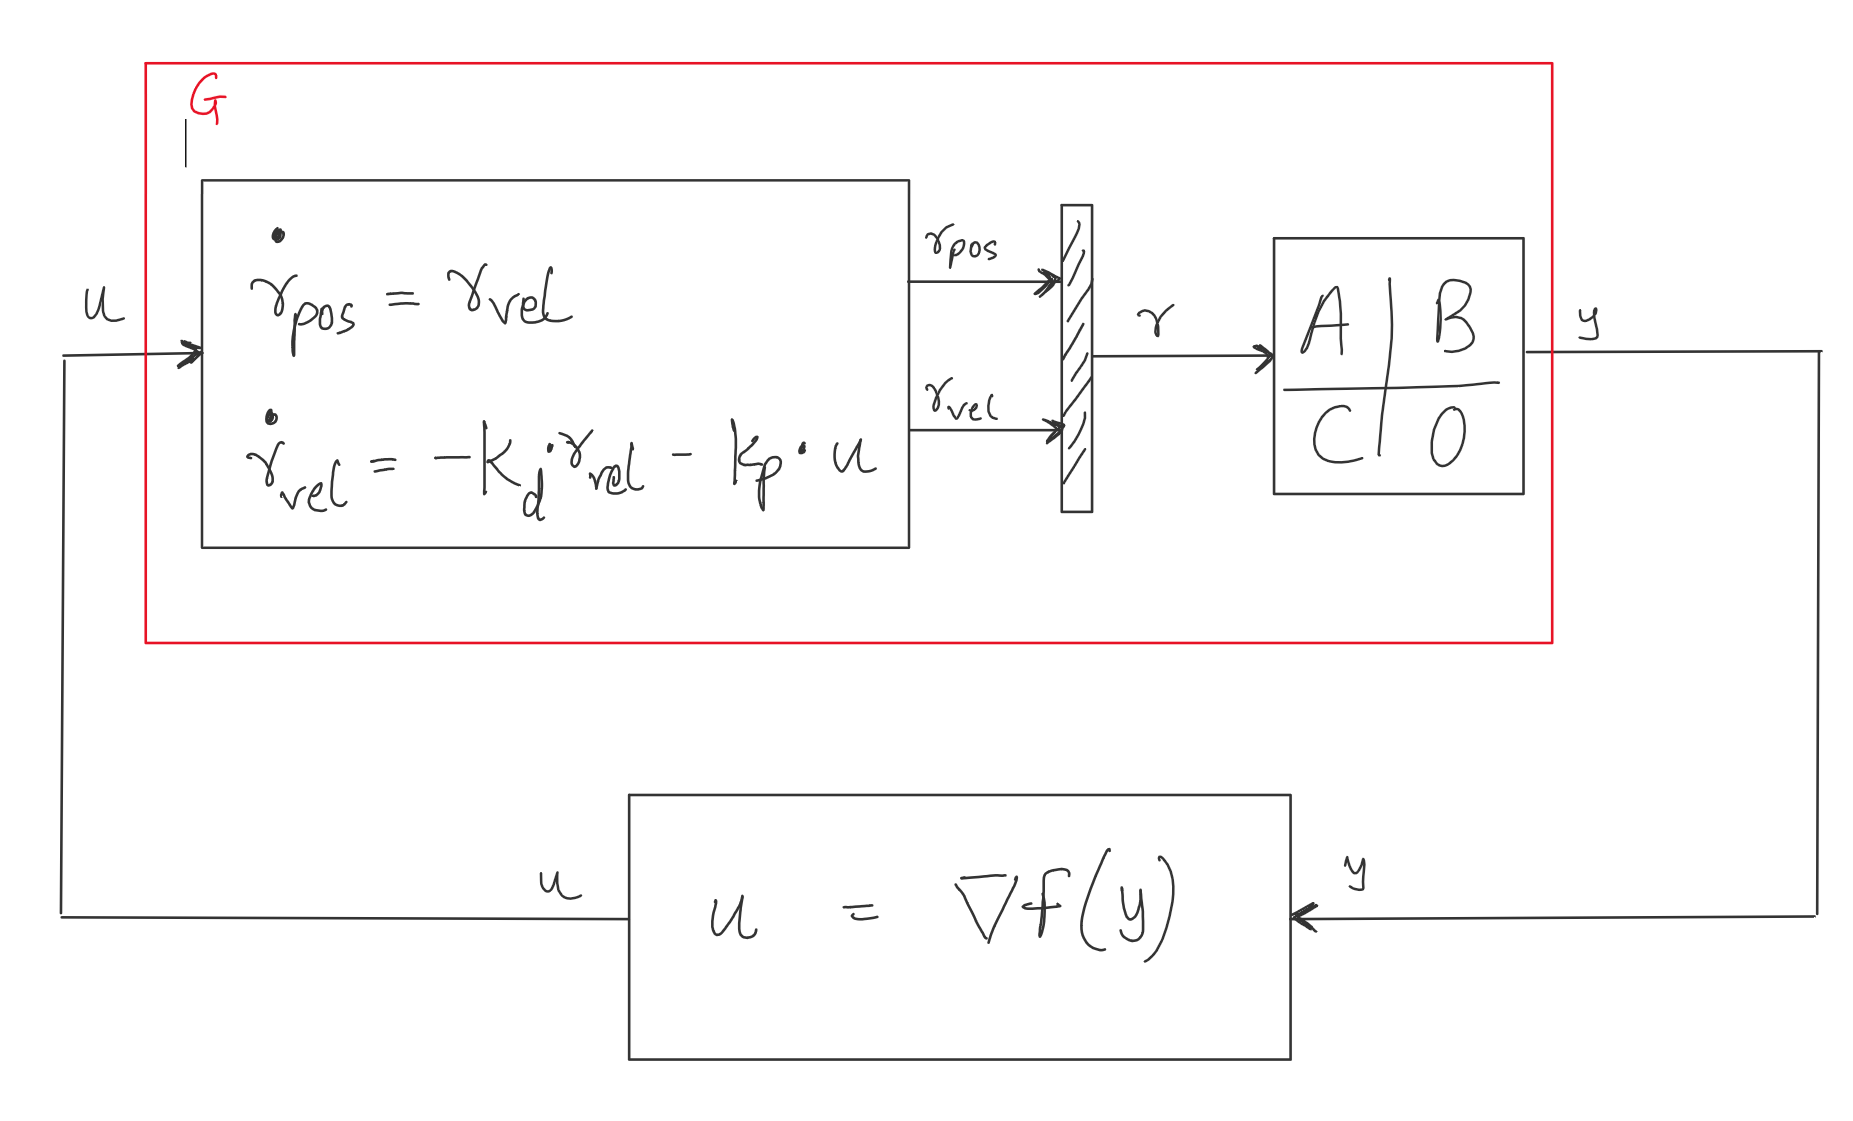
\includegraphics[width=8cm]{figures/Figure_IQC_paper.PNG}
	% This file was created by matlab2tikz.
%
%The latest updates can be retrieved from
%  http://www.mathworks.com/matlabcentral/fileexchange/22022-matlab2tikz-matlab2tikz
%where you can also make suggestions and rate matlab2tikz.
%
\definecolor{mycolor1}{rgb}{0.00000,1.00000,1.00000}%
%
\begin{tikzpicture}

\begin{axis}[%
width=2.361in,
height=2.166in,
at={(0.358in,2.481in)},
scale only axis,
xmin=0,
xmax=18,
xlabel style={font=\color{white!15!black}},
xlabel={L},
ymin=0,
ymax=0.05,
ylabel style={font=\color{white!15!black}},
ylabel={$\alpha$},
axis background/.style={fill=white},
legend style={legend pos=outer north east,legend cell align=left, align=left, draw=white!15!black}
]
\addplot [color=red, line width=1.0pt, only marks, mark=o, mark options={solid, red}]
  table[row sep=crcr]{%
0.3	0.0311279296875\\
1	0.0311279296875\\
5	0.0311279296875\\
6	0.0299072265625\\
7	0.0177001953125\\
8	0\\
9	-1\\
10	-1\\
11	-1\\
12	-1\\
13	-1\\
14	-1\\
15	-1\\
16	-1\\
16.05	-1\\
16.1	-1\\
16.15	-1\\
16.2	-1\\
16.25	-1\\
16.3	-1\\
16.35	-1\\
16.4	-1\\
16.45	-1\\
16.5	-1\\
16.55	-1\\
16.6	-1\\
16.65	-1\\
16.7	-1\\
16.75	-1\\
16.8	-1\\
16.85	-1\\
16.9	-1\\
16.95	-1\\
17	-1\\
17.05	-1\\
17.1	-1\\
17.15	-1\\
17.2	-1\\
17.25	-1\\
17.3	-1\\
17.35	-1\\
17.4	-1\\
17.45	-1\\
17.5	-1\\
17.55	-1\\
17.6	-1\\
17.65	-1\\
17.7	-1\\
17.75	-1\\
17.8	-1\\
17.85	-1\\
17.9	-1\\
17.95	-1\\
18	-1\\
};
\addlegendentry{CC}

\addplot [color=green, dashed, line width=1.0pt]
  table[row sep=crcr]{%
0.3	0.0311279296875\\
0.4	0.0311279296875\\
0.5	0.0311279296875\\
0.6	0.0311279296875\\
0.7	0.0311279296875\\
0.8	0.0311279296875\\
0.9	0.0311279296875\\
1	0.0311279296875\\
5	0.0311279296875\\
10	0.0311279296875\\
15	0.0311279296875\\
16	0.0238037109375\\
16.05	0.023193359375\\
16.1	0.02197265625\\
16.15	0.0213623046875\\
16.2	0.0201416015625\\
16.25	0.0189208984375\\
16.3	0.018310546875\\
16.35	0.01708984375\\
16.4	0.0164794921875\\
16.45	0.0152587890625\\
16.5	0.0140380859375\\
16.55	0.013427734375\\
16.6	0.01220703125\\
16.65	0.0115966796875\\
16.7	0.0103759765625\\
16.75	0.0091552734375\\
16.8	0.008544921875\\
16.85	0.00732421875\\
16.9	0.0067138671875\\
16.95	0.0054931640625\\
17	0.0042724609375\\
17.05	0.003662109375\\
17.1	0.00244140625\\
17.15	0.0018310546875\\
17.2	0.0006103515625\\
17.25	0\\
17.3	-1\\
17.35	-1\\
17.4	-1\\
17.45	-1\\
17.5	-1\\
17.55	-1\\
17.6	-1\\
17.65	-1\\
17.7	-1\\
17.75	-1\\
17.8	-1\\
17.85	-1\\
17.9	-1\\
17.95	-1\\
18	-1\\
};
\addlegendentry{ZF causal}

\addplot [color=blue, dashdotted, line width=1.0pt]
  table[row sep=crcr]{%
0.3	0.0311279296875\\
1	0.0311279296875\\
5	0.0311279296875\\
6	0.0299072265625\\
7	0.0177001953125\\
8	0\\
9	-1\\
10	-1\\
11	-1\\
12	-1\\
13	-1\\
14	-1\\
15	-1\\
16	-1\\
16.05	-1\\
16.1	-1\\
16.15	-1\\
16.2	-1\\
16.25	-1\\
16.3	-1\\
16.35	-1\\
16.4	-1\\
16.45	-1\\
16.5	-1\\
16.55	-1\\
16.6	-1\\
16.65	-1\\
16.7	-1\\
16.75	-1\\
16.8	-1\\
16.85	-1\\
16.9	-1\\
16.95	-1\\
17	-1\\
17.05	-1\\
17.1	-1\\
17.15	-1\\
17.2	-1\\
17.25	-1\\
17.3	-1\\
17.35	-1\\
17.4	-1\\
17.45	-1\\
17.5	-1\\
17.55	-1\\
17.6	-1\\
17.65	-1\\
17.7	-1\\
17.75	-1\\
17.8	-1\\
17.85	-1\\
17.9	-1\\
17.95	-1\\
18	-1\\
};
\addlegendentry{ZF anti-causal}

\addplot [color=mycolor1, line width=1.0pt]
  table[row sep=crcr]{%
0.3	0.0311279296875\\
0.4	0.0311279296875\\
0.5	0.0311279296875\\
0.6	0.0311279296875\\
0.7	0.0311279296875\\
0.8	0.0311279296875\\
0.9	0.0311279296875\\
1	0.0311279296875\\
5	0.0311279296875\\
10	0.0311279296875\\
15	0.0311279296875\\
16	0.0311279296875\\
16.05	0.0311279296875\\
16.1	0.0311279296875\\
16.15	0.030517578125\\
16.2	0.029296875\\
16.25	0.0286865234375\\
16.3	0.0274658203125\\
16.35	0.0262451171875\\
16.4	0.025634765625\\
16.45	0.0244140625\\
16.5	0.023193359375\\
16.55	0.0225830078125\\
16.6	0.0213623046875\\
16.65	0.0201416015625\\
16.7	0.01953125\\
16.75	0.018310546875\\
16.8	0.01708984375\\
16.85	0.0164794921875\\
16.9	0.0152587890625\\
16.95	0.0146484375\\
17	0.013427734375\\
17.05	0.01220703125\\
17.1	0.0115966796875\\
17.15	0.0103759765625\\
17.2	0.0091552734375\\
17.25	0.008544921875\\
17.3	0.00732421875\\
17.35	0.0067138671875\\
17.4	0.0054931640625\\
17.45	0.0042724609375\\
17.5	0.003662109375\\
17.55	0.00244140625\\
17.6	0.001220703125\\
17.65	0.0006103515625\\
17.7	-1\\
17.75	-1\\
17.8	-1\\
17.85	-1\\
17.9	-1\\
17.95	-1\\
18	-1\\
};
\addlegendentry{ZF}

\addplot [color=black, line width=1.0pt, only marks, mark=o, mark options={solid, black}]
  table[row sep=crcr]{%
7.15036762718386	0.0316441620732023\\
7.60555127546399	0.0316441620731976\\
8.06608438061844	0.0316441620732035\\
8.53112887414927	0.0316441620731977\\
9	0.0316441620731958\\
9.47213595499958	0.0316441620732029\\
9.94707355701399	0.0316441620731962\\
10.4244289008981	0.0316441620731959\\
10.9038820320221	0.0316441620731996\\
11.3851648071345	0.0316441620732002\\
11.8680512635611	0.031644162073207\\
12.3523499553598	0.0316441620731978\\
12.837897830943	0.0316441620732007\\
13.3245553203368	0.0316441620731997\\
13.8122023742033	0.0316441620732011\\
14.3007352543677	0.0316441620731969\\
14.7900639201644	0.0316441620731971\\
15.2801098892805	0.0316441620732001\\
15.2801098892805	0.0316441620732001\\
15.3291512169451	0.031644162073202\\
15.3781989601811	0.0316441620732005\\
15.4272530560366	0.0316441620732011\\
15.476313442364	0.0316441620731945\\
15.5253800578078	0.031644162073195\\
15.5744528417925	0.0316441620731975\\
15.6235317345098	0.0316441620731951\\
15.6726166769078	0.0316441620732006\\
15.7217076106782	0.0316441620731991\\
15.7708044782457	0.0316441620731963\\
15.8199072227563	0.0316441620731968\\
15.8690157880665	0.0316441620732018\\
15.9181301187323	0.0316441620732006\\
15.9672501599987	0.0316441620731996\\
16.016375857789	0.0316441620731975\\
16.0655071586947	0.0316441620731986\\
16.1146440099656	0.0316441620731977\\
16.1637863594995	0.0306459324506733\\
16.2129341558325	0.0296357706054901\\
16.26208734813	0.0286272106864285\\
16.3112458861765	0.0276202485903266\\
16.3604097203668	0.0266148802153533\\
16.409578801697	0.0256111014613394\\
16.4587530817554	0.0246089082299991\\
16.5079325127138	0.0236082964252399\\
16.5571170473188	0.0226092619533781\\
16.6063066388837	0.0216118007233945\\
16.6555012412795	0.0206159086471895\\
16.7047008089276	0.0196215816398201\\
16.7539052967911	0.018628815619699\\
16.803114660367	0.0176376065088711\\
16.852328855679	0.0166479502331857\\
16.9015478392689	0.0156598427225296\\
16.9507715681903	0.0146732799110292\\
17	0.0136882577372529\\
17.0492330927517	0.0127047721444192\\
17.0984708049885	0.0117228190805792\\
17.1477130957359	0.010742394498774\\
17.1969599244949	0.00976349435729745\\
17.2462112512353	0.00878611461976904\\
17.2954670363892	0.0078102512553839\\
17.344727240844	0.00683590023905373\\
17.3939918259366	0.00586305755155722\\
17.4432607534465	0.00489171917972533\\
17.4925339855898	0.00392188111657527\\
17.5418114850132	0.00295353936146958\\
17.591093214788	0.00198668992025297\\
17.6403791384037	0.00102132880540657\\
17.6896692197628	5.74520361825287e-05\\
17.7389634231748	-0.000904944361271517\\
17.7882617133505	-0.00186586435376609\\
17.8375640553966	-0.00282531190096338\\
17.8868704148101	-0.003783290955226\\
17.936180757473	-0.00473980546153738\\
17.9854950496473	-0.00569485935733952\\
18.0348132579692	-0.00664845657246534\\
18.0841353494445	-0.00760060102898683\\
18.1334612914436	-0.00855129664113839\\
18.1827910516962	-0.00950054731522072\\
18.2321245982865	-0.010448356949465\\
};
\addlegendentry{Examples in $\Delta_1$}

\addplot [color=black, line width=1.0pt, only marks, mark=asterisk, mark options={solid, black}]
  table[row sep=crcr]{%
14.9273722248242	0.0330736743868692\\
15.3404990089262	0.0345547517944928\\
17.0983319759492	0.0117255854839518\\
16.543288497164	0.0228899773841427\\
16.3221246735849	0.0273976380105542\\
16.1690026664804	0.0305386374015768\\
16.0503713157008	0.0329835817324648\\
17.319486429946	0.00733495581785729\\
17.7116689653864	-0.000372253029782499\\
18.6765413123456	-0.0189191579727348\\
17.8586124663191	-0.00323445286943269\\
};
\addlegendentry{Examples in $\Delta_2$}

\end{axis}

\begin{axis}[%
width=5.833in,
height=4.375in,
at={(0in,0in)},
scale only axis,
xmin=0,
xmax=1,
ymin=0,
ymax=1,
axis line style={draw=none},
ticks=none,
axis x line*=bottom,
axis y line*=left
]
\end{axis}
\end{tikzpicture}%
	\caption{Convergence rate estimates for quadrotor dynamics provided by different multipliers(See Remark \ref{rem:CC_ZF_cusal}) for fields $f\in \mathcal{S}(1,L)$}
	\centering
	%\label{fig:quadrotor_robustness}
\end{figure}
\end{frame}
%%%%%%%%%%%%%%%%%%%%%%%%%%%%%%%%%%%%%%%%%%%%%%%%%%%%%%%%%%%%%%%%%%%%%
\begin{frame}{Example 2: Spectrum of Laplacian unknown}
Assume:
\begin{itemize}
	\item[i] At least one third of total number of agents are leaders
	\item[ii] Maximum degree of all agents is $2$				
	\item[iii] Every agent has an edge with at least one leader
\end{itemize}
\begin{figure}[]	
	\centering
		\begin{overprint}
			\onslide<1>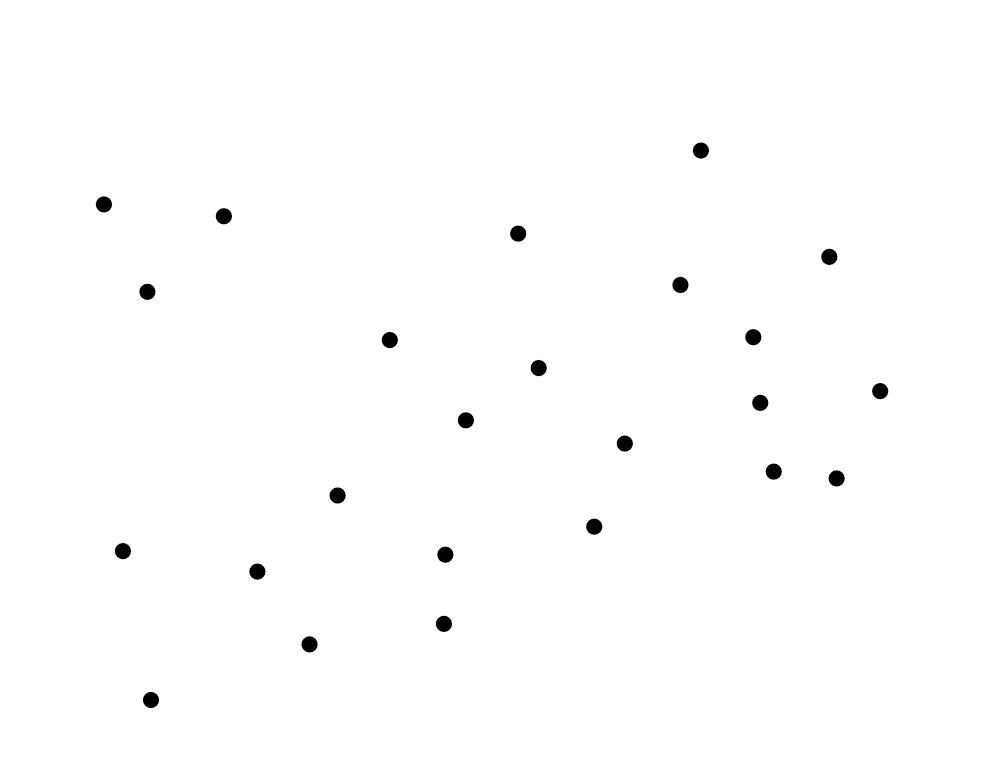
\includegraphics[scale=0.65]{figures/graph_nodes_0.jpg}	
			\onslide<2>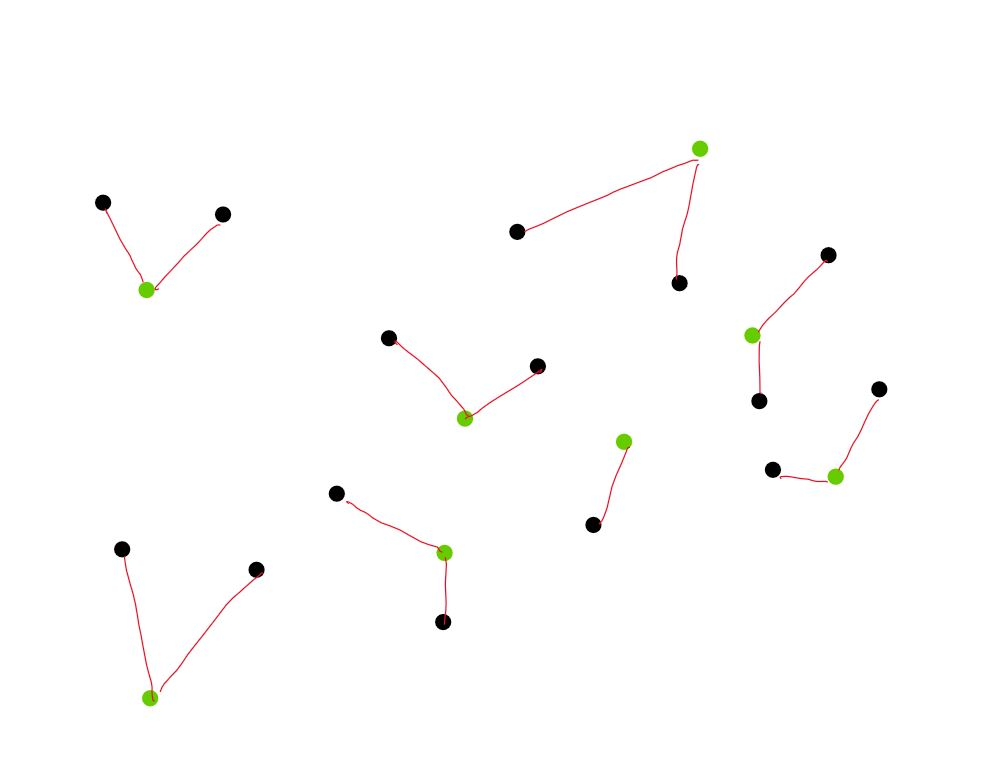
\includegraphics[scale=0.65]{figures/graph_minimal_1.jpg}	
			\onslide<3>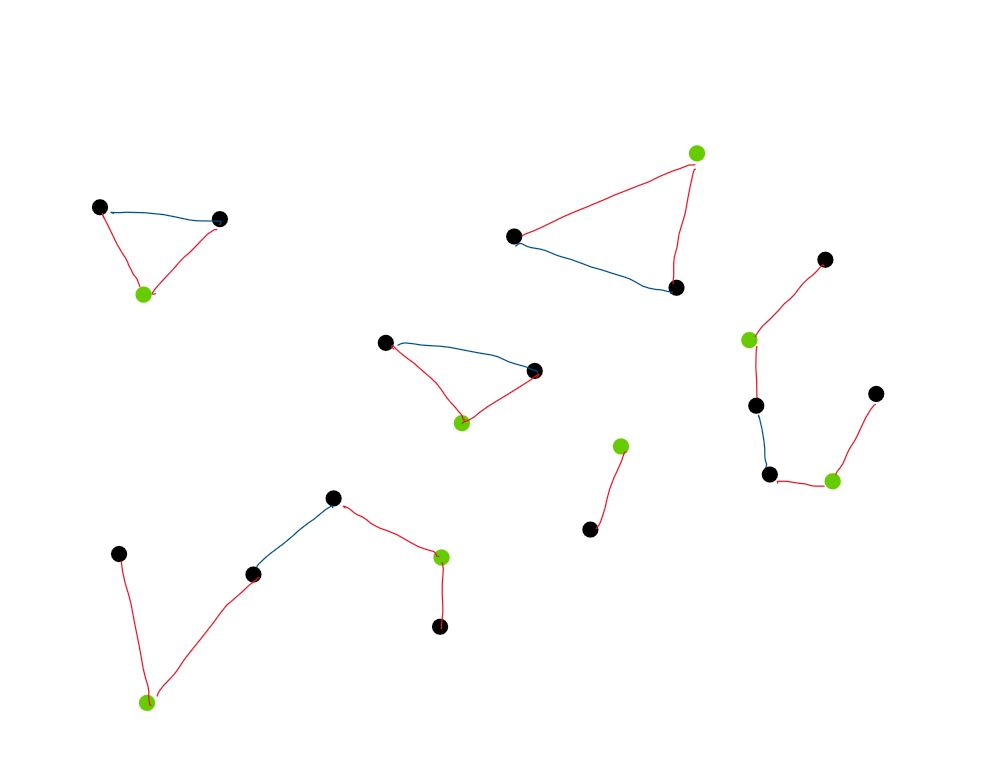
\includegraphics[scale=0.65]{figures/graph_example_2.jpg}	
			\onslide<4>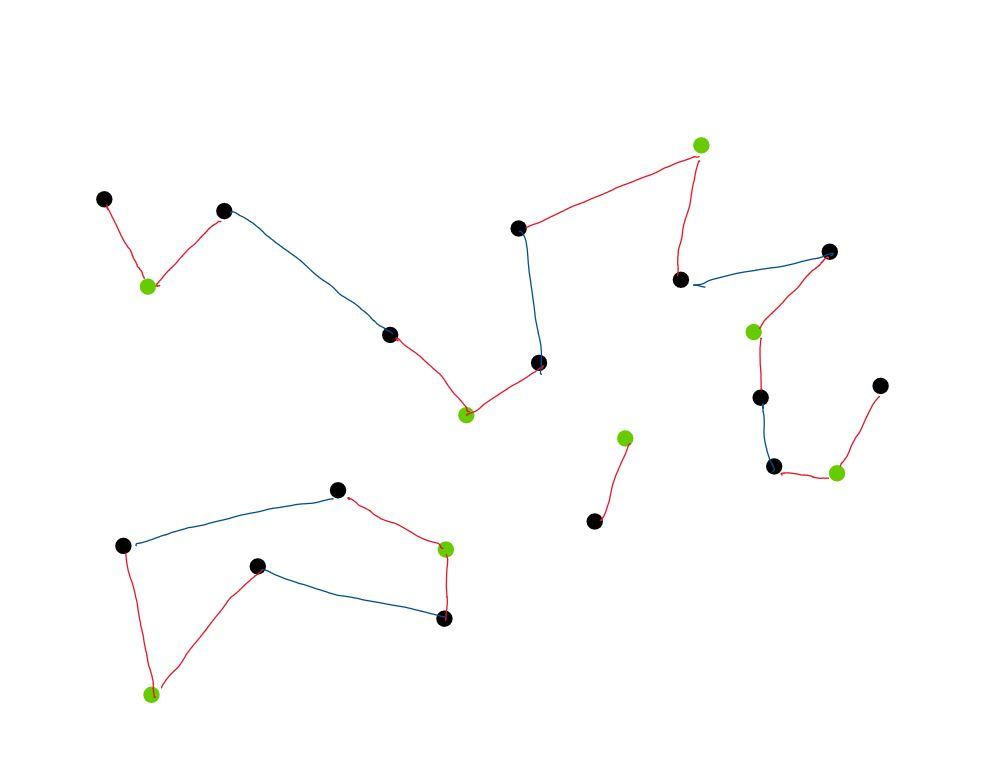
\includegraphics[scale=0.65]{figures/graph_example_3.jpg}
			\onslide<5>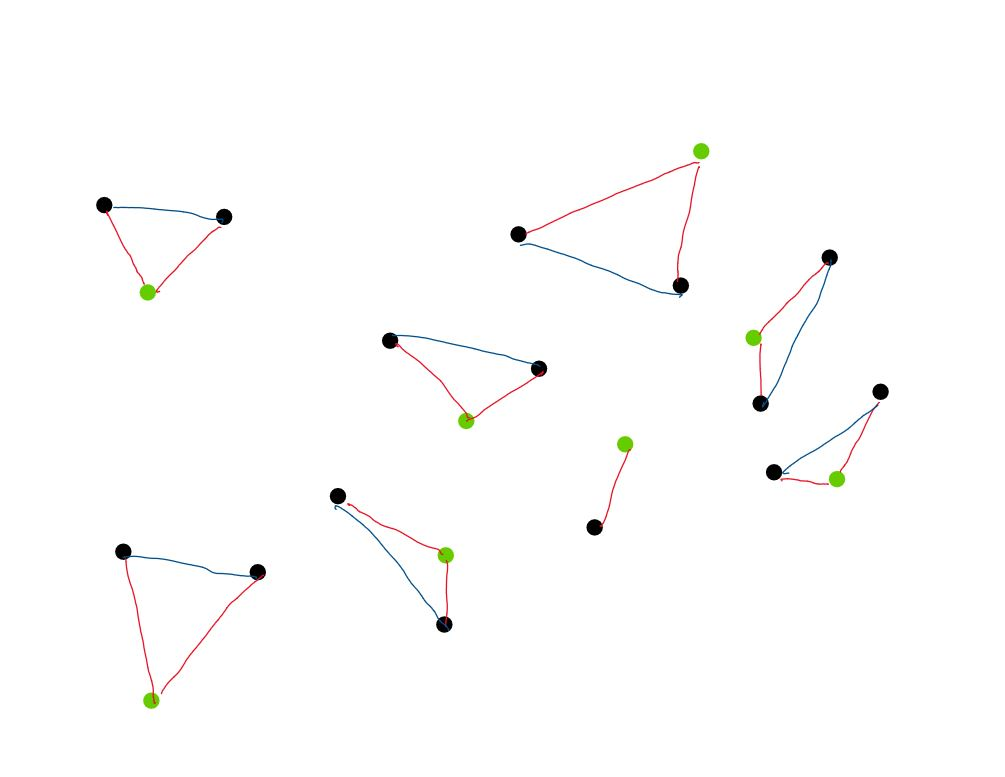
\includegraphics[scale=0.65]{figures/graph_example_4.jpg}	
			\onslide<6->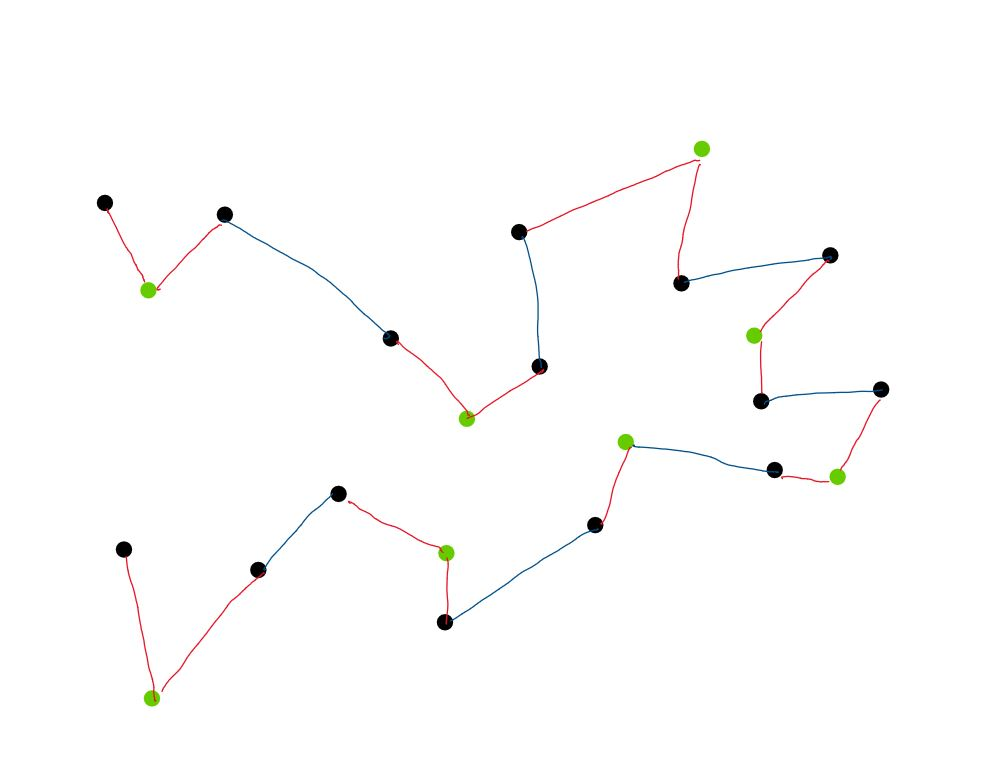
\includegraphics[scale=0.65]{figures/graph_example_5.jpg}	
		\end{overprint}	
\end{figure}
\end{frame}
%%%%%%%%%%%%%%%%%%%%%%%%%%%%%%%%%%%%%%%%%%%%%%%%%%%%%%%%%%%%%%%%%%%%%
\begin{frame}{Example 2: Spectrum of Laplacian unknown}
	Assume:
	\begin{itemize}
		\item[i] At least one third of total number of agents are leaders
		\item[ii] Maximum degree of all agents is $2$				
		\item[iii] Every agent has an edge with at least one leader
	\end{itemize}
\begin{figure}[!htb]
	\centering
	\begin{minipage}{.5\textwidth}
		\centering
		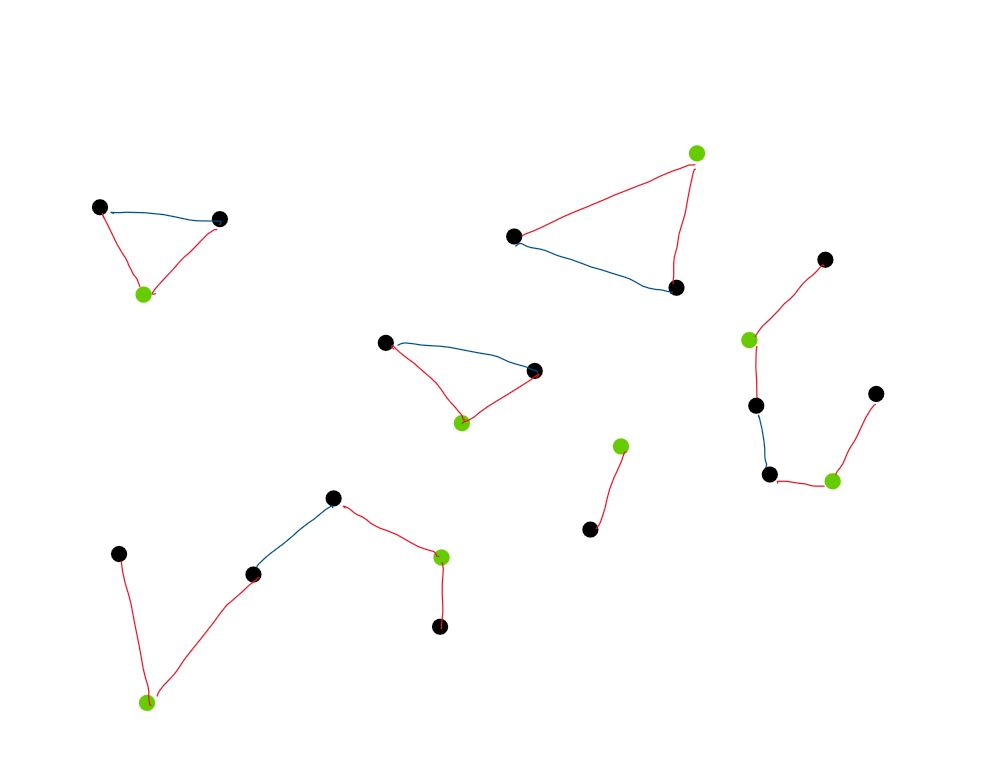
\includegraphics[scale=0.32]{figures/graph_example_2.jpg} \\
		\centering
		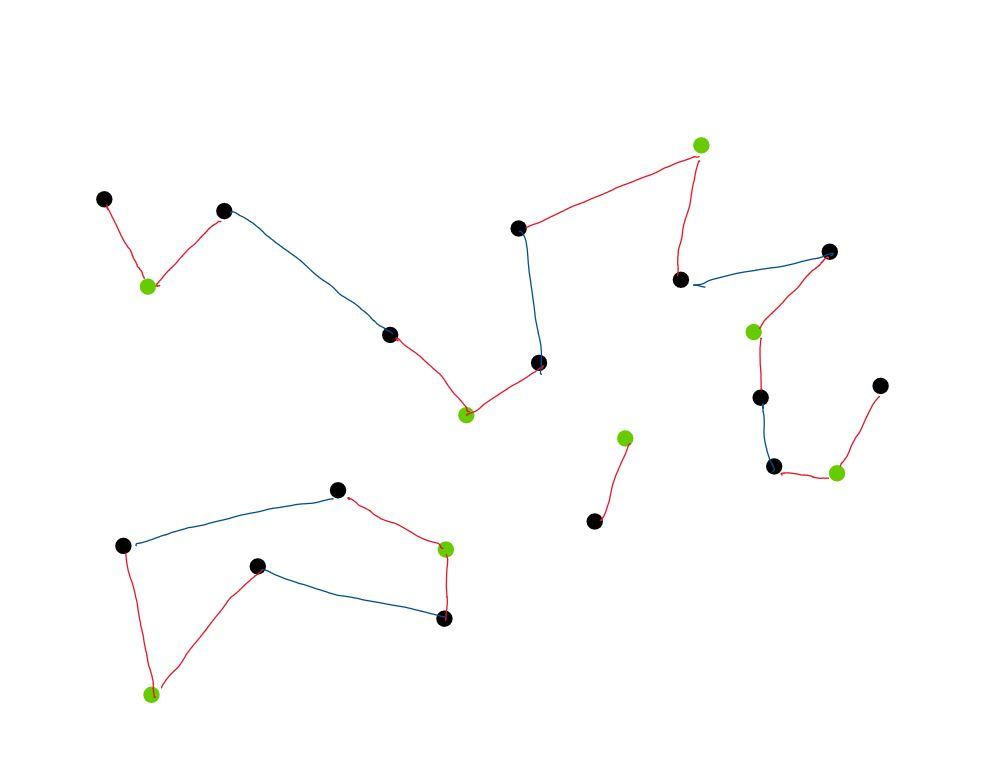
\includegraphics[scale=0.32]{figures/graph_example_3.jpg}
	\end{minipage}%
	\begin{minipage}{0.5\textwidth}
		\centering
		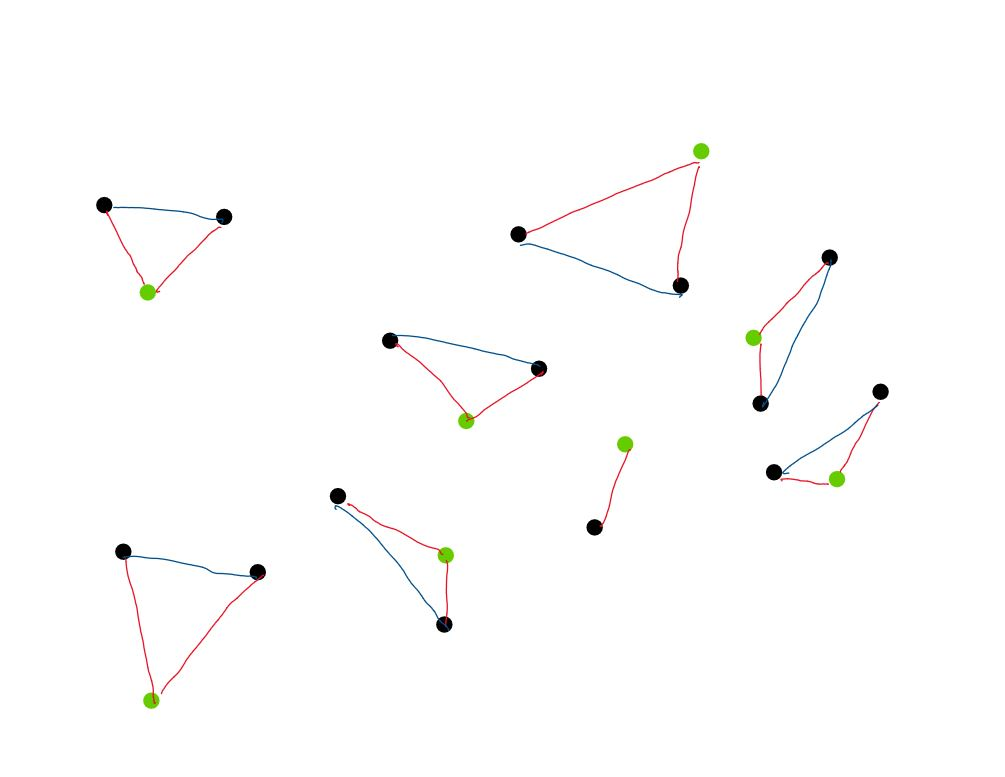
\includegraphics[scale=0.32]{figures/graph_example_4.jpg}\\
		\centering
		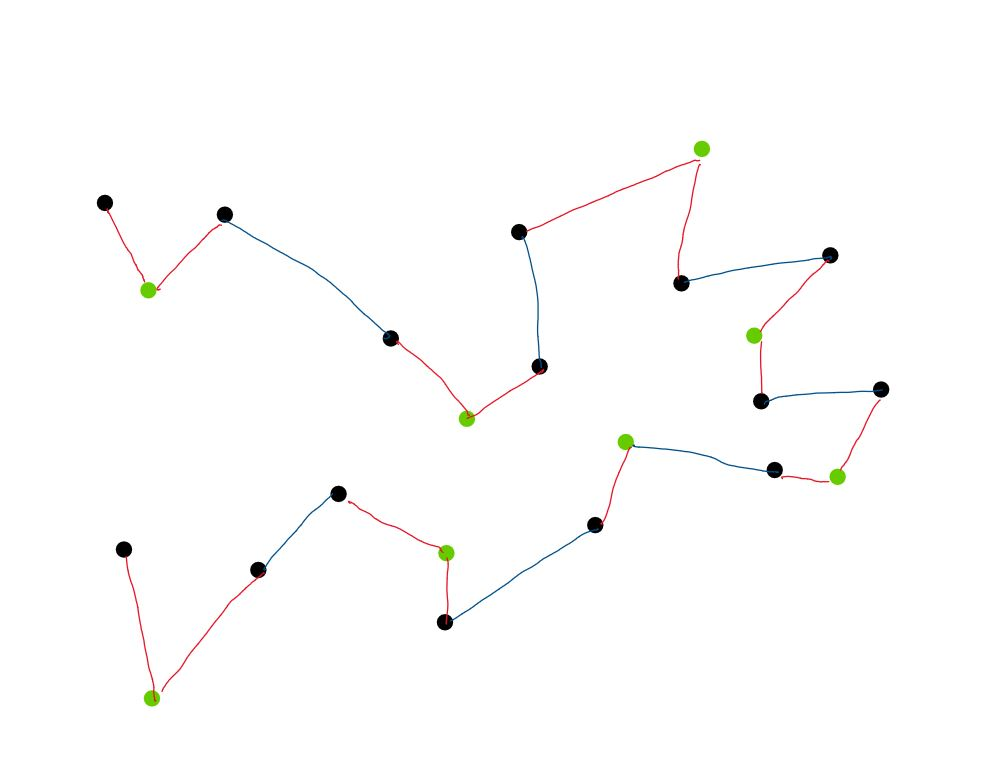
\includegraphics[scale=0.32]{figures/graph_example_5.jpg}
	\end{minipage}
\end{figure}
\end{frame}
%%%%%%%%%%%%%%%%%%%%%%%%%%%%%%%%%%%%%%%%%%%%%%%%%%%%%%%%%%%%%%%%%%%%%
\begin{frame}{Example 2: Spectrum of Laplacian unknown}
	\begin{block}{Setup}
		\begin{itemize}
			\item Linearized quadrotor model + LQR tracking local controller
			\item[1] Conditions on the graph
			\begin{itemize}
				\item[i] At least one third of total number of agents are leaders, i.e., $|\mathcal{V}_l|\geq |\mathcal{V}|$.
				\item[ii] Maximum degree of all agents is $3$				
				\item[iii] Every agent has an edge with at least one leader, i.e., For any $i \in \mathcal{V}$, there is a $j \in \mathcal{V}_l$ such that $(i,j) \in \mathcal{E}$
			\end{itemize}
			\item[2] Let $\psi \in \mathcal{S}(1,L_{\psi})$	
			\item Let $\bar{\Delta}=\{(\mathcal{G},\mathcal{V}_l,\psi): (1),(2)\}$	
			\item Can show: $\bar{\Delta}\subset \Delta_{m,L}$ with $m=0.3$ and $L=L_{\psi}+2*3$				
		\end{itemize}
	\end{block}
\end{frame}
%%%%%%%%%%%%%%%%%%%%%%%%%%%%%%%%%%%%%%%%%%%%%%%%%%%%%%%%%%%%%%%%%%%%%
\begin{frame}{Example 2: Spectrum of Laplacian unknown}
	\begin{figure}[t]
		%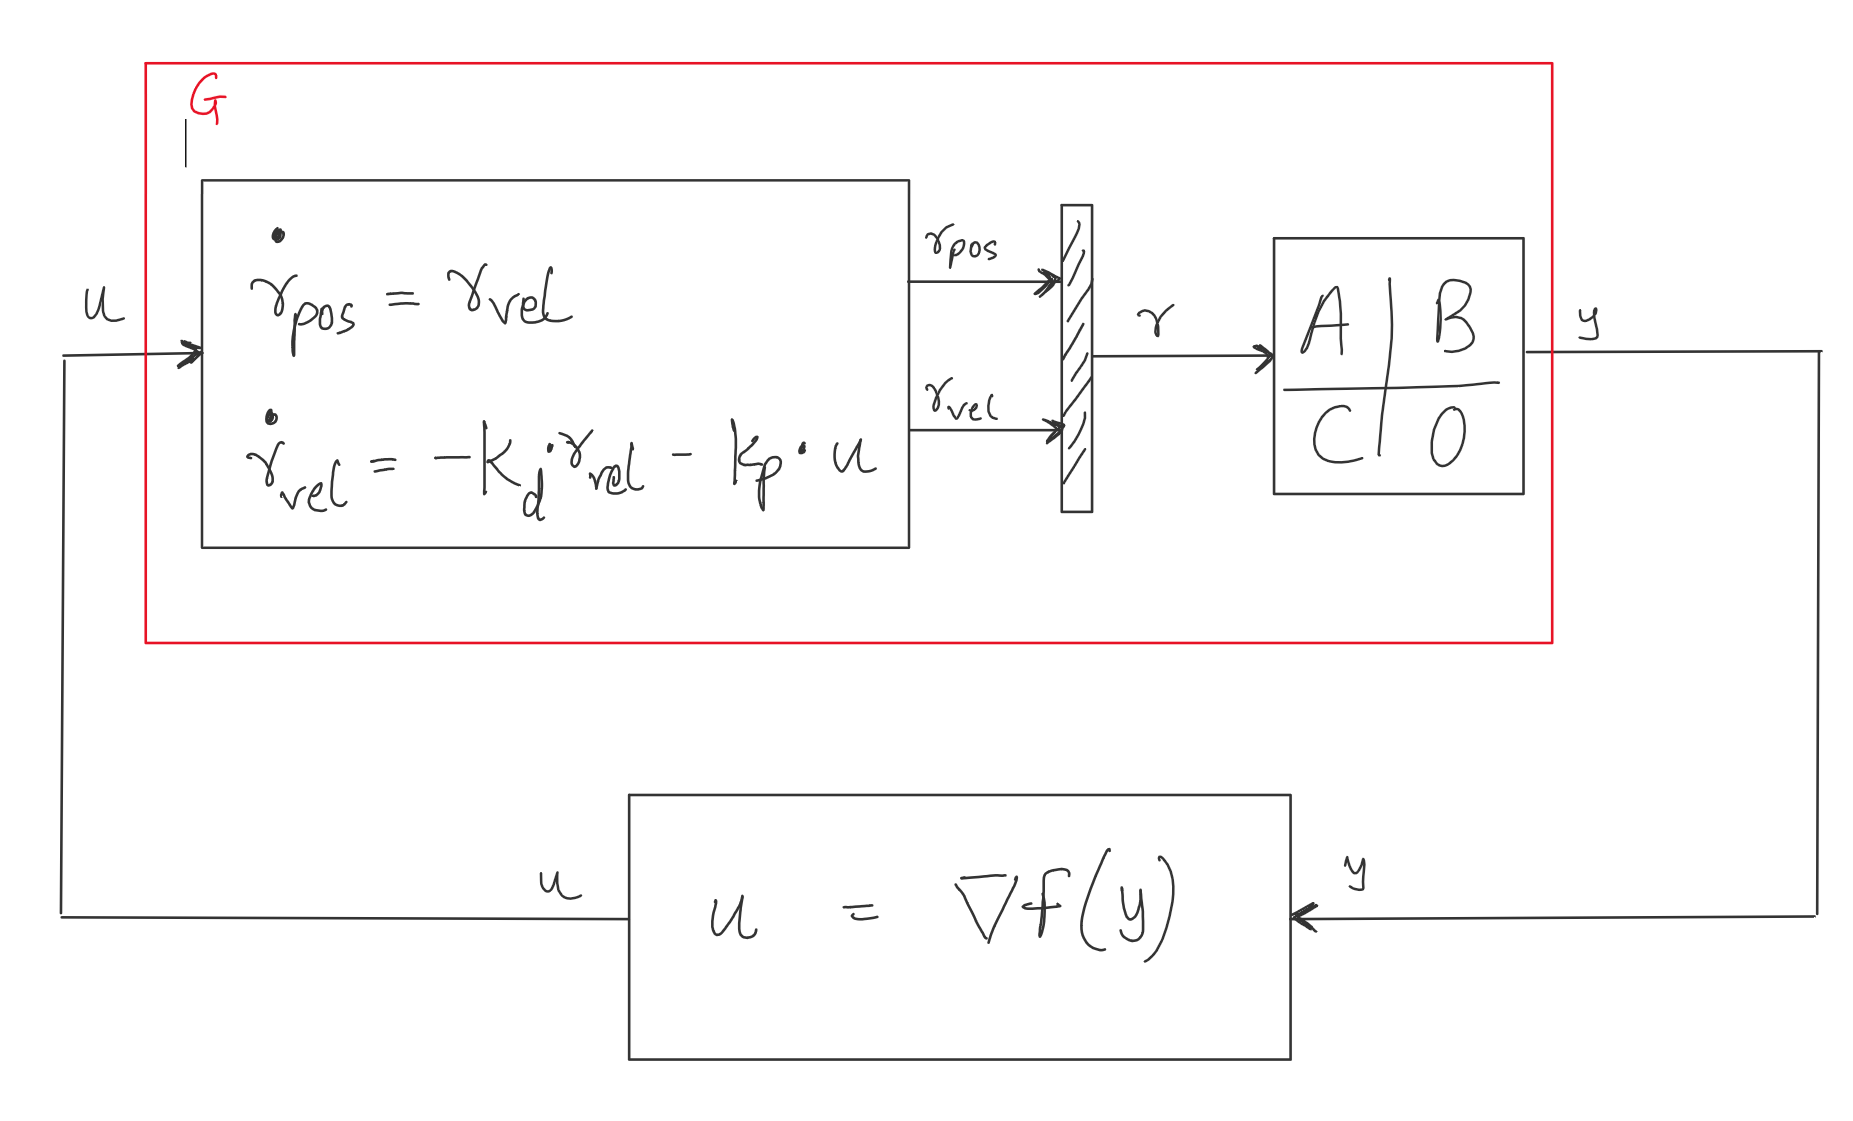
\includegraphics[width=8cm]{figures/Figure_IQC_paper.PNG}
		% This file was created by matlab2tikz.
%
%The latest updates can be retrieved from
%  http://www.mathworks.com/matlabcentral/fileexchange/22022-matlab2tikz-matlab2tikz
%where you can also make suggestions and rate matlab2tikz.
%
\definecolor{mycolor1}{rgb}{0.00000,1.00000,1.00000}%
%
\begin{tikzpicture}

\begin{axis}[%
width=2.361in,
height=2.166in,
at={(0.358in,2.481in)},
scale only axis,
xmin=0,
xmax=16,
xlabel style={font=\color{white!15!black}},
xlabel={$\text{L }\psi$},
ymin=0,
ymax=0.0308429700575454,
ylabel style={font=\color{white!15!black}},
ylabel={$\alpha$},
axis background/.style={fill=white},
legend style={legend pos=outer north east,legend cell align=left, align=left, draw=white!15!black}
]
\addplot [color=red, line width=1.0pt, only marks, mark=o, mark options={solid, red}]
  table[row sep=crcr]{%
1	0.0274658203125\\
2	0.02685546875\\
3	0.0152587890625\\
4	-1\\
5	-1\\
6	-1\\
7	-1\\
8	-1\\
9	-1\\
10	-1\\
11	-1\\
12	-1\\
13	-1\\
14	-1\\
15	-1\\
16	-1\\
17	-1\\
18	-1\\
19	-1\\
};
\addlegendentry{CC}

\addplot [color=green, dashed, line width=1.0pt]
  table[row sep=crcr]{%
1	0.0274658203125\\
2	0.0274658203125\\
3	0.0274658203125\\
4	0.0274658203125\\
5	0.0274658203125\\
6	0.0274658203125\\
7	0.0274658203125\\
8	0.0274658203125\\
9	0.0274658203125\\
10	0.0274658203125\\
11	0.0274658203125\\
12	0.0238037109375\\
13	0.0042724609375\\
14	-1\\
15	-1\\
16	-1\\
17	-1\\
18	-1\\
19	-1\\
};
\addlegendentry{ZF causal}

\addplot [color=blue, dashdotted, line width=1.0pt]
  table[row sep=crcr]{%
1	0.0274658203125\\
2	0.02685546875\\
3	0.0152587890625\\
4	-1\\
5	-1\\
6	-1\\
7	-1\\
8	-1\\
9	-1\\
10	-1\\
11	-1\\
12	-1\\
13	-1\\
14	-1\\
15	-1\\
16	-1\\
17	-1\\
18	-1\\
19	-1\\
};
\addlegendentry{ZF anti-causal}

\addplot [color=mycolor1, line width=1.0pt]
  table[row sep=crcr]{%
1	0.0274658203125\\
2	0.0274658203125\\
3	0.0274658203125\\
4	0.0274658203125\\
5	0.0274658203125\\
6	0.0274658203125\\
7	0.0274658203125\\
8	0.0274658203125\\
9	0.0274658203125\\
10	0.0274658203125\\
11	0.0274658203125\\
12	0.0274658203125\\
13	0.013427734375\\
14	-1\\
15	-1\\
16	-1\\
17	-1\\
18	-1\\
19	-1\\
};
\addlegendentry{ZF}

\addplot [color=black, line width=1.0pt, only marks, mark=o, mark options={solid, black}]
  table[row sep=crcr]{%
1	0.0280390636886659\\
2	0.0280390636886751\\
3	0.0280390636886753\\
4	0.028039063688675\\
5	0.028039063688668\\
6	0.0280390636886774\\
7	0.0280390636886695\\
8	0.0280390636886735\\
9	0.0280390636886776\\
10	0.0280390636886756\\
11	0.028039063688669\\
12	0.0280390636886716\\
13	0.0280390636886746\\
14	0.0280390636886709\\
15	0.0112135608330293\\
16	-0.00823118846524074\\
17	-0.0270745138205892\\
18	-0.045351033302876\\
19	-0.0630930371014014\\
};
\addlegendentry{Examples}

\end{axis}
\end{tikzpicture}%
		\centering
		%\label{fig:quadrotor_robustness}
	\end{figure}
\end{frame}
%%%%%%%%%%%%%%%%%%%%%%%%%%%%%%%%%%%%%%%%%%%%%%%%%%%%%%%%%%%%%%%%%%%%%%
%\begin{frame}{References}
%	\begin{itemize}
%		\item[1] C.  Scherer,  “Dissipativity  and  integral  quadratic  constraints,  tailoredcomputational robustness tests for complex interconnections.” [Online].Available: https://arxiv.org/pdf/2105.07401
%		\item[2]  M.  Fazlyab,  A.  Ribeiro,  M. Morari,  and  V.  M.  Preciado,  “Analysis  ofoptimization algorithms via integral quadratic constraints: Nonstronglyconvex  problems,”SIAM  Journal  on  Optimization,  vol.  28,  no.  3,  pp.2654–2689, 2018.
%		\item[3]  A.  Datar,  P.  Paulsen,  and  H.  Werner,  “Flocking  towards  the  source:Indoor experiments with quadrotors,” in2020 European Control Con-ference (ECC).    IEEE, 5/12/2020 - 5/15/2020, pp. 1638–1643.
%		\item[4]  A.  Attallah,  A.  Datar,  and  H.  Werner,  “Flocking  of  linear  parametervarying  agents:  Source  seeking  application  with  underwater  vehicles,”IFAC-PapersOnLine, vol. 53, no. 2, pp. 7305–7311, 2020.		
%	\end{itemize}
%\end{frame}
%%%%%%%%%%%%%%%%%%%%%%%%%%%%%%%%%%%%%%%%%%%%%%%%%%%%%%%%%%%%%%%%%%%%%%
%\begin{frame}{References}
%	\begin{itemize}		
%		\item[5]  L.  Lessard,  B.  Recht,  and  A.  Packard,  “Analysis  and  design  of  opti-mization  algorithms  via  integral  quadratic  constraints,”SIAM  Journalon Optimization, vol. 26, no. 1, pp. 57–95, 2016.
%		\item[6]  B.  Hu  and  P.  Seiler,  “Exponential  decay  rate  conditions  for  uncertainlinear systems using integral quadratic constraints,”IEEE Transactionson Automatic Control, vol. 61, no. 11, pp. 3631–3637, 2016.
%		\item[7]  R. A. Freeman, “Noncausal zames-falb multipliers for tighter estimatesof  exponential  convergence  rates,”  in2018  Annual  American  ControlConference (ACC).    IEEE, 6/27/2018 - 6/29/2018, pp. 2984–2989.
%		\item[8]  J.   Veenman   and   C.   W.   Scherer,   “Stability   analysis   with   integralquadratic  constraints:  A  dissipativity  based  proof,”  in52nd  IEEEConference on Decision and Control, 2013, pp. 3770–3775.
%	\end{itemize}
%\end{frame}
%%%%%%%%%%%%%%%%%%%%%%%%%%%%%%%%%%%%%%%%%%%%%%%%%%%%%%%%%%%%%%%%%%%%%%
%\begin{frame}{References}
%	\begin{itemize}		
%		\item[9]  J.    Zhang,    P.    Seiler,    and    J.    Carrasco,    “Noncausal    fir    zames-falb  multiplier  search  for  exponential  convergence  rate.”  [Online].Available: https://arxiv.org/pdf/1902.09473
%	\end{itemize}
%\end{frame}
%%%%%%%%%%%%%%%%%%%%%%%%%%%%%%%%%%%%%%%%%%%%%%%%%%%%%%%%%%%%%%%%%%%%%
\begin{frame}{}
\begin{center}
    \huge{Thank you}
\end{center}
\end{frame}
%%%%%%%%%%%%%%%%%%%%%%%%%%%%%%%%%%%%%%%%%%%%%%%%%%%%%%%%%%%%%%%%%%%%%
%%%%%%%%%%%%%%%%%%%%%%%%%%%%%%%%%%%%%%%%%%%%%%%%%%%%%%%%%%%%%%%%%%%%%
%\begin{frame}{Decomposing flocking dynamics under quadratic fields}
%	\begin{figure}[t]
%		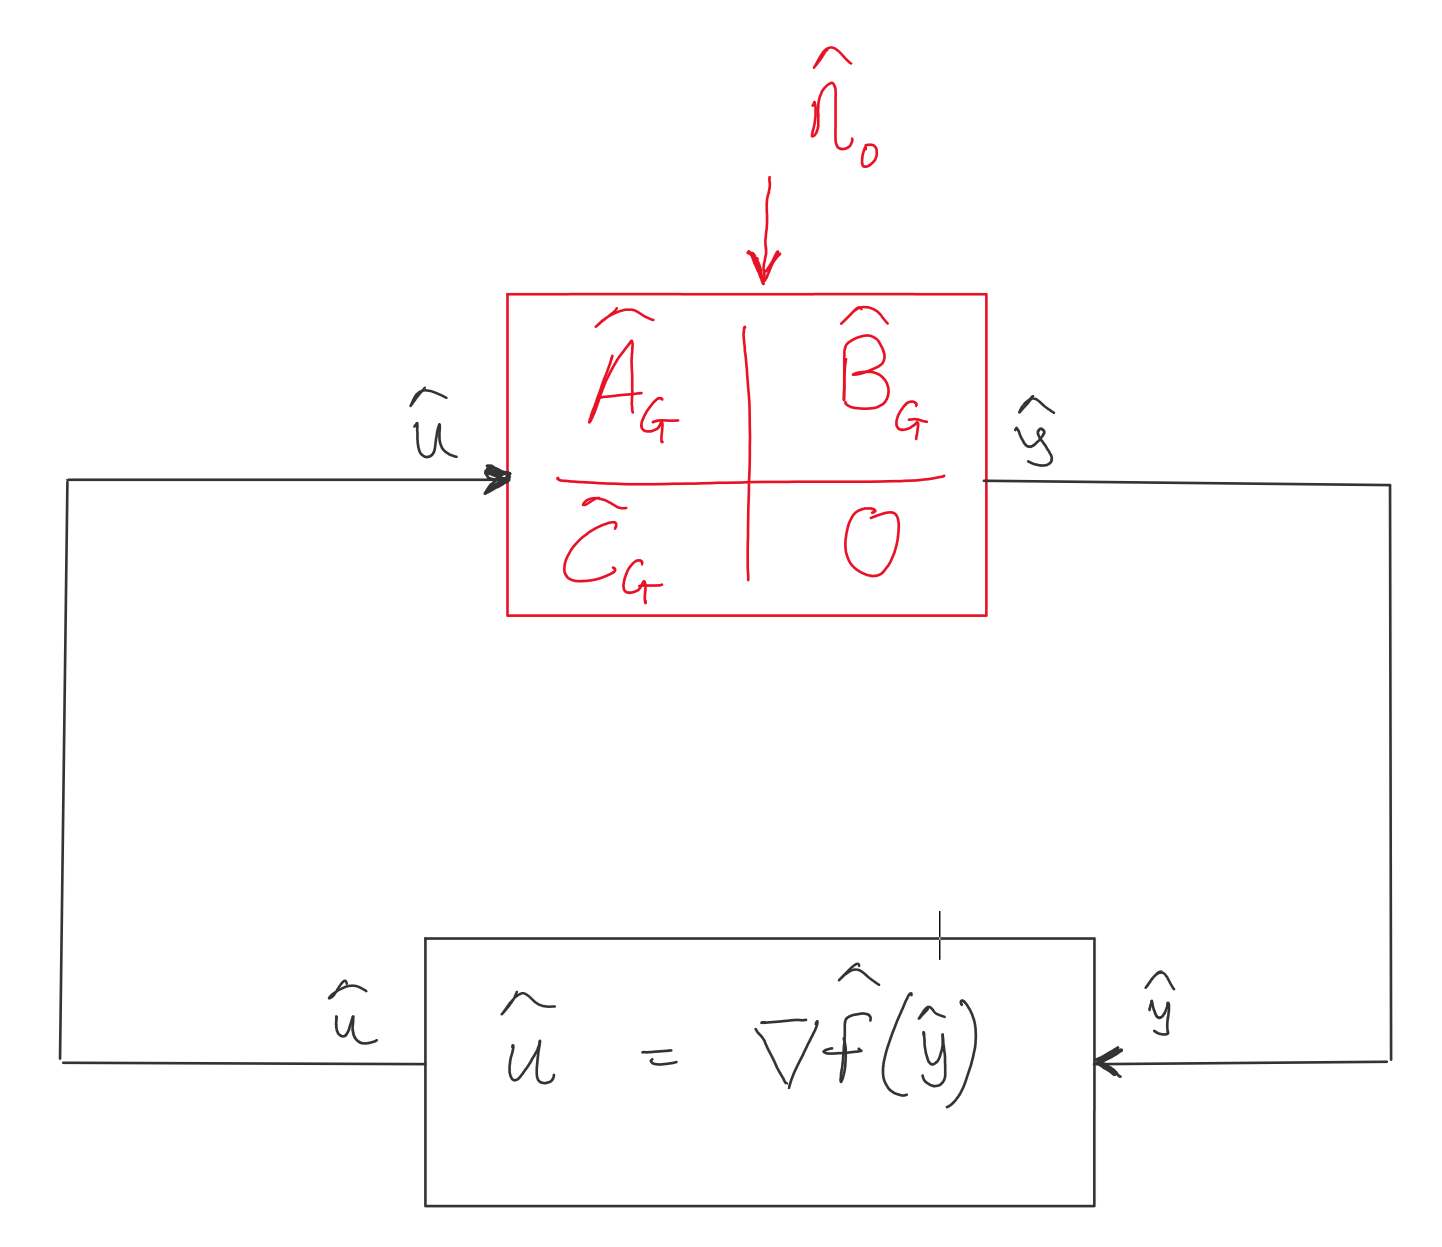
\includegraphics[width=6cm]{figures/loop_multiple_agents.PNG}
%		%\input{figures/quadrotor_trajectory}
%		\caption{Block diagram}
%		\centering
%		%\label{fig:Figure_IQC_paper}
%	\end{figure}
%	\begin{equation} \label{eq:flocking_dynamics}
%		\begin{split}
%			\Dot{\hat{\eta}}(t)&=(I_N \otimes A_G)\hat{\eta}(t) + (I_N \otimes B_G)\hat{u}(t),\\
%			\hat{y}(t)&=(I_N \otimes C_G)\hat{\eta}(t) \\
%			\hat{u}(t)&=\nabla \hat{f}(\hat{y}(t))-\nabla \mathcal{V}(\hat{y}(t))-(\mathcal{L}\otimes I_d)\Dot{\hat{y}}(t).
%		\end{split}
%	\end{equation}
%\end{frame}
%%%%%%%%%%%%%%%%%%%%%%%%%%%%%%%%%%%%%%%%%%%%%%%%%%%%%%%%%%%%%%%%%%%%%%
%\begin{frame}{Decomposing flocking dynamics under quadratic fields}
%	\begin{block}{Averaging out state, input and output:Center Of Mass(COM)} $\eta_c=\textnormal{avg}(\hat{\eta})$, $y_c=\textnormal{avg}(\hat{y})$, $u_c=\textnormal{avg}(\hat{u})$
%	\end{block}
%	\begin{block}{Quadratic fields (Linear gradients)}
%		\begin{itemize}
%			\item $f(y)=y^T Q y + c^Ty + d \implies \nabla f (y)=2 Qy + c$
%			\item $\textnormal{avg}(\nabla \hat{f}(\hat{y}))=\nabla f (\textnormal{avg}(\hat{y}))=\nabla f(y_c)$
%		\end{itemize}
%	\end{block}
%	\begin{block}{Averaging dynamics \eqref{eq:flocking_dynamics}}
%		\begin{itemize}
%			\item $\textnormal{avg}((I_N \otimes A_G)\hat{\eta})=A_G{\eta_c}$ (Similary for $B_G$ and $C_G$)
%			\item $\textnormal{avg}(\nabla \mathcal{V}(\hat{y}))=\mathbf{0}$,$\textnormal{avg}((\mathcal{L}\otimes I_d))=\mathbf{0}$ 
%		\end{itemize}
%	\end{block}
%	\begin{equation}\label{eq:COM_dynamics}
%		\begin{split}
%			\Dot{\eta_c}(t)
%			% &=\frac{1}{N}(\mathbf{1}_N^T \otimes I_{n_\eta})((I_N \otimes A_G)\hat{\eta}(t) + (I_N \otimes B_G)\hat{u}(t)),\\
%			% &=\frac{1}{N}(\mathbf{1}_N^T \otimes A_G)\hat{\eta}(t)+ \frac{1}{N}(\mathbf{1}_N^T \otimes B_G )\hat{u}(t)),\\
%			&=A_G \eta_c + B_G u_c,\\
%			\hat{y}_c(t)
%			% &=\frac{1}{N}(\mathbf{1}_N^T \otimes I_{d})(I_N \otimes C_G)\hat{\eta}(t) \\
%			&= C_G \eta_c\\
%			\hat{u}_c(t)&=\nabla f (y_c).
%		\end{split}
%	\end{equation}
%\end{frame}
%%%%%%%%%%%%%%%%%%%%%%%%%%%%%%%%%%%%%%%%%%%%%%%%%%%%%%%%%%%%%%%%%%%%%
%\begin{frame}{Abstracting to a Mathematical Problem}	
%\begin{block}{Problem Statement:}
%Design distributed control algorithms for large networks of mobile robots such that the group shows a desirable behavior.
%\end{block}
%\begin{itemize}
%	\item Desirable behaviors we consider:
%	\begin{itemize}
%		\item Consensus and/or Formation stabilization
%		\item Flocking with/without source seeking
%	\end{itemize}	
%	\item Complexity in solving the problem can stem through:
%	\begin{itemize}
%		\item Complicated dynamics of individual agents
%		\item Commplicated Interconnection structure and intractible design algorithms for large networks
%	\end{itemize}
%\end{itemize}
%\end{frame}
%%%%%%%%%%%%%%%%%%%%%%%%%%%%%%%%%%%%%%%%%%%%%%%%%%%%%%%%%%%%%%%%%%%%%
%\begin{frame}{Approaching the problem: Divide and Conquer}
%\begin{block}{Available literature on}
%\begin{itemize}
%	\item Control of single complex agent dynamics (e.g LPV, control of differetially flat systems, dynamic inversion) 
%	\item Distributed control of large networks of "simple" agent dynamics (e.g single and double intergrators) -> Consensus and Flocking algorithms
%\end{itemize}
%\end{block}	
%\begin{block}{Consider as building blocks}
%\begin{itemize}
%	\item Closed-loop system $G_{\textnormal{cl}}$ with some guaranteed performance measure such as the induced $\mathcal{L}_2-\mathcal{L}_2$ or  $\mathcal{L}_2-\mathcal{L}_{\infty}$ norms
%	\item Consensus or Flocking algorithms for "simple" systems
%\end{itemize}
%\end{block}
%\end{frame}
%%%%%%%%%%%%%%%%%%%%%%%%%%%%%%%%%%%%%%%%%%%%%%%%%%%%%%%%%%%%%%%%%%%%%
\end{document}

